% !Mode:: "TeX:UTF-8"
\documentclass[type=doctor,openany,pifootnote]{shuthesis}
% 选项:
%  type=[master|profmaster|doctor], % 必选
%  secret,                          % 可选 (如果论文需要保密, 这一项需要打开)
%  pifootnote,                      % 可选(建议打开)
%  openany|openright,               % 可选 (章首页是右开还是任意开, 默认是右开)
%  nocolor                          % 提交最终版本时请打开此选项
\usepackage{shuthesis}
% \usepackage{newtxmath}
\graphicspath{{figures/}}

\begin{document}
\frontmatter
\shusetup{
  %%%%%%%% 1. 配置里面不要出现空行. 2. 不需要的配置信息可以删除. %%%%%%%%%%%
  secretlevel={公开},             % 秘级
  % 中文信息
  ctitle={基于大模型的智能问答系统关键技术研究与应用},
  cdisciplines={工学},
  cdepartment={机电工程与自动化学院},
  cmajor={电子信息},
  cauthor={***},
  csupervisor={***},
  id={********},
  catalognumber={TP391},
  cdate={2025 年 7 月},
  coverdate={\zhdigits{2025}年\zhnumber{7}月},
  % 英文信息
  etitle={Research and application of key technologies of Question Answering system based on large language models},
  edisciplines={Engineering},
  edepartment={School of Mechatronic Engineering and Automation},
  emajor={Electronic and Information Engineering},
  eauthor={***},
  esupervisor={***},
  edate={july, 2025}
}

% 中英文摘要和关键字
\begin{cabstract}
    随着大模型的基础理论研究日趋成熟,其优秀的多模态理解能力和生成能力被应用于众多技术框架和复杂场景工业辅助设计、多参数控制系统运维决策等垂直领域中。然而在大模型的实际应用场景中仍面临许多困难和挑战。大模型本身的优越性能依赖于其庞大的参数及计算资源,并且在实际使用的推理框架中还涉及文本嵌入、知识检索等其他功能模块,这些降低了大模型推理框架的时效性。同时大模型在数据分析领域的应用也有一定的局限,尤其是在表格数据推理方面,大模型对表格数据的推理能力有限,无法直接处理复杂的表格数据,从而造成明显的幻觉问题。此外,针对包含反馈控制的智能系统,由于缺乏足够的训练数据,进一步限制了其推理能力的提升。面对以上问题,本文针对大模型在检索增强生成( Retrieval-Augmented Generation ,RAG)技术框架的应用展开研究,重点研究模型轻量化压缩、表格数据推理优化等关键问题,提高大模型推理效率和对于表格数据的推理能力。并在水利水库调度领域开拓了应用场景,设计并实现了该领域下的基于本地知识库的大模型智能反馈交互系统。本文的主要工作归纳如下: 

    1、针对一种文本编码网络——循环神经网络,提出一种基于本征正交分解(Proper Orthogonal Decomposition, POD)的动力学系统模型压缩方法,通过循环神经网络隐藏状态的低维投影,将模型参数量与计算量分别压缩至原始模型的34.4\%与25.6\%,精度损失控制在5\%以内,并将传统动力学方法引入神经网络中,提高了其可解释性。
    
    2、针对大模型对结构化表格数据推理的局限性,设计多级表格检索和推理框架,结合Agent代理思想及SQL代码生成技术,将复杂数值计算转化为可执行程序,并构建检索-优化-生成的循环自纠错机制,优化了推理质量。
    
    3、针对数字孪生灌区目前存在的智能反馈交互系统缺失,无法适应调度系统升级需求等问题,设计并实现了数字孪生灌区多功能智能知识库,结合RAG技术为智能反馈交互系统提供本地知识支撑。通过建立业务规则库来支撑业务场景的规则适配,规范和约束水利业务管理行为。

    4、为验证上述基于本征正交分解的动力学系统模型压缩方法、多级表格检索和推理框架等方法在实际场景中的优化效果,设计并实现了基于知识库的智能反馈交互系统。将检索增强生成技术与本地知识库技术结合并成功应用于水库调度、灌溉管理等场景,提升了水利水库调度领域的智能化水平。
    \end{cabstract}
    
    \ckeywords{大模型,模型压缩,表格数据推理,智能反馈交互系统}
    
    \begin{eabstract}
        As research on large language models matures, their strong multimodal understanding and generation capabilities have been applied to various technical frameworks and complex industrial scenarios, such as industrial-assisted design, multi-parameter control system operation and maintenance decision-making. However, several challenges remain in the practical application of large language models.
        The superior performance of large language models depends on their massive parameters and computing resources. In addition, other functional modules such as text embedding and knowledge retrieval are involved in the reasoning framework, reducing its timeliness. Moreover, large language models have limitations in data analysis, especially in tabular data reasoning. They can't directly handle complex tabular data, leading to significant hallucination problems. Furthermore, for intelligent systems with feedback control, insufficient training data restricts the improvement of reasoning capabilities.
        To address these issues, this thesis focuses on the application of large language models within the Retrieval-Augmented Generation (RAG) technical framework, aiming to enhance reasoning efficiency and tabular data reasoning capabilities through model lightweight compression and tabular data reasoning optimization. It also explores the hydrological reservoir scheduling field by developing an intelligent feedback interaction system based on a local knowledge base. The main contributions are as follows:
        
        1、A Proper Orthogonal Decomposition (POD)-based dynamical system model compression method for Recurrent Neural Networks (RNNs) is proposed. It reduces model parameters and computations to 34.4\% and 25.6\% of the original, with a precision loss of less than 5\%, and improves interpretability by incorporating traditional dynamical methods.

        2、A multi-level tabular retrieval and reasoning framework is designed to address the limitations of large language models in structured tabular data reasoning. By integrating the Agent proxy concept and SQL code generation, complex numerical calculations are transformed into executable programs. Additionally, a cyclic self-correction mechanism of retrieval-optimization-generation is established to enhance reasoning quality.

        3、To address the issues of missing intelligent feedback interaction systems in digital twin irrigation districts and their inability to meet the upgrading needs of scheduling systems, a multifunctional knowledge base for digital twin irrigation districts is designed and implemented. It provides local knowledge support for the intelligent feedback interaction system through RAG technology. Meanwhile, a business rule library is established to support business scenario rule adaptation and standardize and constrain water conservancy business management practices.

        4、To verify the practical optimization effects of the above mentioned POD based dynamical system model compression method for RNNs, the multi-level tabular retrieval and tabular reasoning framework, a knowledge based intelligent feedback interaction system is developed. It combines RAG with local knowledge base technologies, successfully applied to reservoir scheduling and irrigation management, enhancing intelligence in the field.
        
    \end{eabstract}
    
    \ekeywords{ Large Language Models, Model Compression, Table Data Reasoning, Intelligent Feedback Interaction System}
    
\makefirstpage                         % 生成带有学校 logo 的封面
\makecover

\tableofcontents                       % 目录

% % !Mode:: "TeX:UTF-8"
\begin{denotation}[2.5cm]
\item[$\mathcal{T}$] 张量
\item[$H$] 超图
\item[$\mathcal{A}(H)$] 超图 $H$ 的邻接张量
\item[$\mathcal{L}(H)$] 超图 $H$ 的拉普拉斯张量
\item[$\mathcal{Q}(H)$] 超图 $H$ 的无符号拉普拉斯张量
\item[$\rho$] 谱半径
\item[$G$] 图
\item[$\kappa$] 连通度
\item[$\chi$] 染色数
\item[$\Delta$] 最大度
\item[$\delta$] 最小度
\end{denotation}
                % 符号对照表

% 正文部分
\mainmatter
% !Mode:: "TeX:UTF-8"
\chapter{绪论}
\label{cha:intro}

本章首先介绍了基于大模型智能反馈交互系统的选题背景及研究意义,接着介绍了大模型表格数据推理及反馈系统的国内外研究现状,通过国内外相关研究进展引出了本文的主要研究内容及工作要点,为后续章节主要研究工作的论述做好铺垫,最后介绍了论文的结构。
 
\section{课题研究的目的和意义}
检索增强生成(Retrieval-Augmented Generation, RAG)技术,实现了从外部知识库中检索相关信息并将其作为上下文输入到大语言模型中,从而生成更准确、更相关的答案。该系统主要包含两个阶段:首先,使用检索模型根据用户问题检索相关文档;然后,以检索到的上下文为基础,利用大语言模型生成最终的回答。

近年来,大模型反馈系统和大模型表格推理技术在金融分析、社会服务和专家咨询等垂直领域加速落地,推动了人工智能在智能交互与信息处理领域的应用,助力国家数字经济和智能化发展的战略目标。该方向的研究紧密结合中国“数字中国”建设和《新一代人工智能发展规划》的建设需求,具有重要的理论与实践价值。通过研究大模型反馈系统,可提升自然语言理解和生成技术在政务、医疗、金融等领域的实际应用能力,提高信息交互效率;而大模型表格推理技术则能实现对结构化数据的自动解析与推断,为复杂的决策支持、数据分析和业务管理提供高效和精准的技术解决方案。

在大模型反馈系统推理及部署相关技术中,由于推理框架中的各种模型参数较大,需要较高的存储和运算能力,而对于实时提供问题回答的反馈系统,推理速度显得尤为重要。所以,模型的轻量化压缩技术是提高模型响应速度,改善用户体验的关键技术。大模型的反馈系统在如金融、医疗和科研等众多领域有广泛的应用\cite{1024008988.nh,1024532352.nh,1024651093.nh,1024744443.nh,1024917032.nh},针对反馈系统的开发,确定的应用场景极为关键。

在常微分方程神经网络(Ordinary Differential Equation Neural Network)\cite{chenNeuralOrdinaryDifferential}的提出下,动力学系统微分方程和神经网络的结合进入大众视野。研究者逐渐将神经网络与动力学系统相联系,利用动力学系统中成熟且丰富的方法处理神经网络模型。借助动力学系统模型降阶的方法应用于神经网络的模型压缩中,能够提出新的模型压缩方法并验证两个领域存在联系,提高神经网络模型的理论可解释性,并为后续神经网络的理论研究提供思路。同时在大模型的嵌入层应用压缩算法,提高模型的推理速度,进而提高智能反馈交互系统的相应速度。

大模型反馈系统的开发离不实际工程应用场景。开发完整的反馈系统需要成熟的向量数据库存储及检索技术及框架,大模型检索增强推理技术应用部署框架及网络部署框架,来提高基于本地知识库的高并发性、可扩展性和高响应速度。为提高大模型的表格数据推理能力,还需要额外引入Agent代理思想,运用数据库技术提升对数据的处理能力。来满足针对特殊场景下不同结构文本数据的理解能力,有效解决面对表格数据问题的幻觉问题从而提高回答质量。

基于以上背景及目的意义,本文研究了基于本征正交分解的循环神经网络模型压缩算法和大模型表格数据推理框架,设计了面向水利水库调度领域的基于本地知识库的大模型智能反馈交互系统,最后完成了知识库及其大模型反馈系统的落地部署。



\section{国内外研究概况}
\subsection{RAG系统研究概况}
LLM(Large Language Model,大语言模型)\cite{kuzmanChatGPTBeginningEnd2023,heAnnoLLMMakingLarge2023,weiFinetunedLanguageModels2022,chenLabelfreeNodeClassification2023,chungScalingInstructionFinetunedLanguage2022,xuWizardLMEmpoweringLarge2023}的出现为NLP(Nature Language Process,自然语言处理)领域任务带来了巨大改变与提升。OpenAI在2020年和2023年发布的GPT类大模型\cite{kuzmanChatGPTBeginningEnd2023,floridiGPT3ItsNature2020},以及2023年发布的Llama\cite{touvronLLaMAOpenEfficient2023}系列大模型和Gemini\cite{teamGeminiFamilyHighly2024}等大模型在多项NLP任务中都达到了前所未有的高度。甚至在一些任务中的表现超过了人类\cite{luFiniteLayerNeural2020,hendrycksMeasuringMassiveMultitask2021}。
尽管大语言模型在许多任务中都展现了强大的能力,但其仍存在一些需要改进的地方。例如,在面对复杂问题或特定领域时,模型可能生成不准确的信息\cite{zhangHowLargeLanguage2023}。当用户的查询超出模型训练数据范围,或者需要最新信息时,模型的知识储备可能显得不足 \cite{kandpalLargeLanguageModels2023}。这种局限性在生成式人工智能的实际应用中尤为突出,仅依赖于不透明的大语言模型通常无法满足生产环境的要求。虽然通过微调可以使传统神经网络适应特定领域,但这种方法需要大量计算资源和专业技术,且在动态更新的信息环境中适应性较差。

大语言模型的知识储备主要分为参数化知识和非参数化知识。参数化知识通过训练储存在模型的权重中,体现了对训练数据的理解及泛化能力,而非参数化知识则存在于外部知识库中,如向量数据库,可随时更新以增强模型对最新或领域特定信息的利用能力。完全基于参数化知识的模型有一些局限,例如无法完全记忆训练数据中的所有信息,尤其是稀有或特定的知识点。此外,模型参数不可实时更新,导致随着时间推移其知识逐渐过时;同时,参数规模的增加也显著提升了训练与使用的计算成本。

为克服这些问题,研究\cite{gaoRetrievalAugmentedGenerationLarge2024}提出了一种结合参数化与非参数化知识的策略,即检索增强生成(Retrieval-Augmented Generation, RAG)。RAG 方法结合了信息检索系统与序列到序列生成模型\cite{gaoRetrievalAugmentedGenerationLarge2024},通过端到端优化实现知识的高效整合。在检索环节,广泛采用了如密集通道检索(Dense Passage Retrieval, DPR)\cite{karpukhinDensePassageRetrieval2020} 等技术,而生成环节则利用小型模型进行端到端训练或调优\cite{izacardFewshotLearningRetrieval2022}。随着大语言模型的兴起,这种方法逐渐演变为一种提升模型性能的主流技术。尽管大语言模型在多项语言任务中表现卓越,其在知识更新与数据相关性等方面的不足仍影响了在知识密集型任务中的表现\cite{yaoEditingLargeLanguage2023,bangMultitaskMultilingualMultimodal2023}。研究\cite{heGRetrieverRetrievalAugmentedGeneration2024}表明,将 RAG 融入情境内学习(In-Context Learning, ICL)中,能够动态从外部知识库中获取信息,从而提升回答的准确性与相关性,并有效降低生成错误的可能性。通过结合生成能力与灵活的信息检索模块,RAG 为解决大语言模型的知识不完整性提供了一种高效的解决方案,广泛应用于提升模型可靠性与实用性。

原始的RAG框架只由必要组件组成如下图\ref{基础RAG结构}所示,将知识文件以向量数据库的形式存储,通过对比用户查询与数据库中向量的相似度,筛选出相关性最大的数据作为提示词,再与查询一同由大模型进行推理。

\begin{figure}[!htbp]
  \centering
  \includegraphics[scale=0.6]{图1.1.png}
  \bicaption[基础RAG结构]{基础RAG结构}[Basic RAG Structure]{ Basic RAG Structure}
  \label{基础RAG结构}
\end{figure}

这种原始的RAG系统存在一些局限性会限制系统的回答质量,如检索的准确性,通过传统向量相似度的方法有时不能在数据库中找到最合适的数据最为提示词,有研究者就此提出过利用大模型检索并结合知识图谱代替向量数据库的KG-RAG\cite{wangKnowledgeGraphPrompting2023}方法来改善这一弱点。知识库的分块程度等问题也是决定系统回答质量的关键问题,针对检索环节有代表性的成果有:

DenseX\cite{chenDenseRetrievalWhat2024}深入探讨了在密集检索(Dense Retrieval)中,不同检索粒度对检索性能和下游任务的影响。他们发现,传统的检索单元如文档、段落或句子的选择对性能有显著影响,并提出“命题”,一种新的检索单元,这种单元能够以简洁、自包含的自然语言格式表达明确的事实。通过对比文档、段落和命题三种粒度的检索效果,论文发现命题检索单元在检索性能和下游问答任务中显著优于其他粒度。引入了一种新的检索单元,以及证明了其在提升检索精度和问答系统性能方面的潜力。具体来说,命题检索单元能够更精确地捕捉到与查询相关的信息,减少了无关细节的干扰,从而提高了检索的准确性和效率。

PKG\cite{luoAugmentedLargeLanguage2023}方法提出了Parametric Knowledge Guiding (PKG)框架,这是一个创新的解决方案,旨在通过知识引导模块增强大型语言模型(LLMs)在特定领域任务中的表现,而无需调整模型参数。该框架基于开源的“白盒”语言模型,允许模型离线存储所需知识。它的主要贡献是解决了LLMs在特定领域任务中数据暴露不足的问题,并且通过保持模型参数不变,避免了数据隐私泄露的风险。PKG框架通过提供一个知识引导模块,使得LLMs能够在不直接访问私有数据的情况下,利用外部知识源来提高其在特定任务上的表现。这种方法不仅提高了模型的性能,还保持了数据的隐私性和模型的透明度。

在EAR\cite{luoDivideConquerEntailmentaware2023}中,作者关注于多跳问题的答案检索,并提出了文本蕴含关系在检索证据时的重要性。他们将任务分解为语义文本相似性和推理相似性检索两个子任务,并提出了EAR和EARnest模型。这些模型不仅在HotpotQA数据集上显著优于单一检索模型,而且还展示了在处理复杂问答任务时考虑多样化相关性信号的有效性。它不仅提高了模型在多跳问答任务中的性能,而且还通过考虑文本蕴含关系,增强了模型对证据之间复杂关系的理解和推理能力。这种方法通过将复杂的检索任务分解为更小、更易管理的子任务,然后联合优化这些子任务的结果,从而提高了整体的检索性能。

G-Retriever\cite{heGRetrieverRetrievalAugmentedGeneration2024}是一种针对文本图普理解和问答的检索增强生成方法。G-Retriever通过将任务表述为奖收集斯坦纳树优化问题,有效处理超出LLMs上下文窗口大小的文本图普,并减轻幻觉问题。这项工作的亮点在于它为文本图普任务提供了一种新的检索增强生成框架,并且在多个领域的文本图普任务上显示出优越的性能。G-Retriever方法通过结合图神经网络和大型语言模型的优势,不仅提高了对文本图普的理解能力,还增强了模型在复杂问答任务中的表现。这种方法通过优化图结构,使得模型能够更有效地检索和利用图中的信息,从而提高了问答的准确性和效率。

KnowledGPT\cite{wangKnowledGPTEnhancingLarge2023}框架连接LLMs与知识库(KBs),促进知识的检索和存储。KnowledGPT使用思维提示程序生成KBs的搜索语言,并提供个性化KB中知识存储的能力。这项工作的创新点在于它不仅提高了LLMs回答需要世界知识的问题的能力,而且还提供了个性化知识存储的解决方案。KnowledGPT通过整合外部知识源,使得LLMs能够访问和利用更广泛的知识,从而提高了模型在各种任务中的表现。这种方法通过提供检索和存储知识的能力,使得LLMs能够更好地适应和满足用户的个性化需求。
UPRISE\cite{chengUPRISEUniversalPrompt2023}中提出了一个轻量级且多功能的检索器,它自动为给定的零样本任务输入检索提示。UPRISE在跨任务和跨模型场景中展示了普遍性,并在实验中减轻了幻觉问题。展示了在不同规模的LLMs上进行测试的能力,以及在提高零样本任务性能方面的潜力。UPRISE通过自动检索适合特定任务的提示,减少了对模型特定微调和任务特定提示工程的需求。这种方法通过提供一个通用的解决方案,提高了LLMs在零样本任务中的泛化能力和性能。
\begin{table}[htb]
  \centering
  \begin{minipage}[t]{0.8\linewidth}
    \bicaption[常见检索优化方法]{常见检索优化方法}[Common Methods For Improving Search Performance]{Common Methods For Improving Search Performance}
    \label{tab:template-files}
    \begin{tabularx}{\linewidth}{lXXXXX}
      \toprule[1.5pt]
      {\heiti 方法}  & {\heiti 检索来源} & {\heiti 数据类型} & {\heiti 检索粒度}  & {\heiti 检索过程}                                    \\\midrule[1pt]
      DenseX & Wikipedia &文本 &主题 &一次 \\
      EAR & 数据集    &文本 &句子 &一次                               \\
      UPRIZE & 数据集    &文本 &句子 &一次                                             \\
      PKG & 大模型    &表格、文本 &块 &一次                                           \\
      KnoledGPT & 数据集    &知识图谱 &三联体 &多次                                        \\
      G-Retriever & 数据集    &文本图谱 &子图 &一次\\
      \bottomrule[1.5pt]
    \end{tabularx}
  \end{minipage}
\end{table}
\subsection{大模型表格数据推理研究概况}
对于自然语言处理的任务大多都是直接由输入得到输出的端到端系统完成的\cite{devlinBertPretrainingDeep2018,raffelExploringLimitsTransfer2020}。这类端到端的方法灵活方便,但是缺少可解释性和鲁棒性。与这种方法相对的是通过生成代码等符号语言并执行的,具有中间过程的方法,输出结果是由外部接口驱动的。这种方法相对于端到端方法有更好的可解释性。大模型的文本推理能力已经得到了充分的证实\cite{kuzmanChatGPTBeginningEnd2023,floridiGPT3ItsNature2020,liuGPTUnderstandsToo2023},但对于结构化的表格数据仍存在明显的幻觉问题,受限于大模型的训练方式,很难通过端到端的方式训练模型对表格数据的推理能力,所以研究这门利用Agent代理的思想,通过中间步骤弥补对数据理解能力的不足。主要思想是将大模型不擅长的数据理解能力转化成代码生成能力。

PoT(Program of Thoughts)\cite{chenLargeLanguageModels2023,chenProgramThoughtsPrompting2023}先受到利用大模型解决数学问题的启发,利用多种上下文学习方法评估在少样本下大模型对表格的推理能力,发现尽管效果上不如SOTA模型,但是实验结果表明在处理表格推理时,提示词学习能大大提高大模型的推理能力。之后根据Chain-of-thought (CoT)\cite{weiChainofthoughtPromptingElicits2022}分步推理的思路,针对复杂的涉及数据计算的自然语言处理问题,提出了将自然语言理解与复杂计算分开进行推理的Program-of-thought (PoT)。根据提示词设置,将问题转化为可执行的代码,如Python,再将程序通过解释器计算结果,将计算好的数据和问题再由CoT的方法输出最终回答,避免了理解自然语言和计算数据同时进行而导致的准确度下降问题。

该方法主要提出将PoT方法作为常规CoT的中间过程,利用更具体的编程语言和程序解释器计算复杂的计算问题,减轻模型语言理解问题的压力,提高推理准确性。文中处理表格作为输入时,将表格转化为线性的文本字符串表示,表格结构由特殊的字符区分,可以有由python包直接读取为表格形式进行计算。

RAJKUMAR \cite{rajkumarEvaluatingTexttoSQLCapabilities2022}跟随PoT\cite{chenProgramThoughtsPrompting2023}的思路,验证大模型(Codex, GPT-3)对于Text-to-SQL任务的生成能力。文章采用了Spider文本生成SQL语言数据集作为基线,在零样本、少样本和提示词学习三种情况下进行实验。Spider由表格查询的自然语言形式和SQL语言形式的字符串对组成。如,

Return the maximum and minimum number of cows across all farms.

	SELECT max(Cows) , min(Cows) FROM farm
    
通过评估模型的输出SQL与标签SQL的匹配程度等评估模型的Test-to-SQL能力。文章只评估了模型由文本生成SQL程序的能力,没有过多框架的提出。

Dater\cite{yeLargeLanguageModels2023}指出直接使用Chain-of-Thought分解问题会导致模型出现幻觉问题,导致子问题会出现与材料不符的情况,所以需要更加复杂的子问题分解方法。文章中将分析表格数据分为两个主要部分。首先为了解决Chain-of-Thought分解含数字问题会导致幻觉的情况,提出了parsing-execution-filling策略,通过大模型将复杂问题分解为多个在数字部分有缺省的子问题,再生成能够填补缺省的SQL程序,执行程序并填补缺省。总结来讲就是根据问题来生成子问题和能够完成子问题的SQL程序,该方法能在解决数字不准确的情况的同时增加其可解释性。然后针对输入的表格有时过于庞大和冗余的情况,文中使用大模型通过行列索引的方式来提取包括关键信息的子表格,最后将子问题和子表格再次输入给大模型得到问题的答案。该方法主要调用三次大模型分别为,生成子表格、生成子问题和根据子表格和子问题输出最终答案。其中在生成子问题时通过生成SQL程序并执行来完成子问题中的计算部分。

CHAIN-OF-TABLE\cite{wangChainofTableEvolvingTables2024}将表格形式的数据和提示词输入给大模型使其从操作池中选择对表格的操作(operation)再将该操作与表格等提示词输入给大模型得到操作的输入参数(args),再根据得到的操作和参数修改表格,将前一步的操作保存至chain列表中作为下一次重复操作的提示词,直到将表格简化到最容易回答问题的形式,再次调度大模型输出问题回答。该方法循环调度大模型,每次循环调度两次,分别生成对表格的处理操作和操作的输入参数,每次循环都会改变一次表格并扩充操作列表chain作为下一次的输入,当模型输出结束符号[E]时结束循环,再单独调用一次大模型生成最终回答。

该法方法再次细化SQL生成过程和子表格生成过程,相较于Dater\cite{yeLargeLanguageModels2023}一步生成子表格,该方法逐步运行SQL语句将原始表格变化成最终表格,相较之下因为中间可视化部分增加,拥有了更好得可解释性。在生成SQL程序的步骤也基于前面的方法进行了细分,由直接根据表格和问题生成SQL程序改为先生成具体的SQL操作,再生成操作中具体的参数,组合生成需要执行的SQL程序。

Binder\cite{chengBindingLanguageModels2023}提出在符号语言中绑定语言模型,与CoT\cite{wangChainofTableEvolvingTables2024}的思路相同,希望通过增加中间步骤的方法增强大语言模型解读表格信息的能力。文章将过程分为两步,解析和执行:解析指将问题表格等提示词输入给大模型,大模型根据提示词生成对应的符号语言,如SQL、Python等(与直接可执行的代码不同,会有类似伪代码的部分,需要额外调用大模型来完成任务)。执行阶段是指将生成的符号语言和表格通过代码解释器(有时需要调用大模型)生成新的子表格,再由子表格和问题通过大模型生成最后的回答。其中对于复杂的不能够由原始表格直接得到的信息,需要额外调用API,利用大模型增加列或直接进行端到端的回答问题。

解析阶段生成的代码根据问题的复杂程度可以分为可以直接生成表格的SQL程序,和需要额外调度大模型来辅助的SQL伪代码(伪代码部分通常用一个函数表示),最终都生成子表格用于最后调度大模型回答问题。与chain-of-table\cite{wangChainofTableEvolvingTables2024}不同的是,Binder中提出的方法只通过一次大模型调用生成代码并可能在执行过程中调用第二次模型生成表格来完成问题,CoT\cite{wangChainofTableEvolvingTables2024}是多次分布生成SQL代码,每次只执行一步并生成新的表格,每步分为两次调用模型生成代码,循环直到表格最简化回答问题。

以上几种框架的提出根本原因是大模型对于表格信息中同时存在的文本推理和数字计算能力不强,尤其是数字推理能力,所以引入SQL等编码语言将对数字的计算能力转化为对代码的生成能力。同时为了提高大模型的准确性和可解释性,尽量将每次调用大模型执行的任务简化细分,模型解决的问题越简单,生成的答案准确性越高;中间步骤输出越多,可解释性就越强。主要思路为两个部分,一是将自然语言理解与数值计算分开;二是将生成任务尽可能地细分,如何解决以上两个问题为大语言模型理解表格数据的关键。

Data-Copilot\cite{zhangDataCopilotBridgingBillions2023}受到前人工作的启发,结合之前工作与结论,主张大模型不应该直接处理数据,而应该充当大脑,创建适当的界面工具来管理和利用数据,以人为中心的方式呈现有价值的信息。提出了Data-Copilot,一种可视化数据分析框架,提供多种工具调用接口。针对不同问题和计算机语言,提出接口的设计和调度策略,并将Data-Copilot应用于股市数据分析中,评估其数据分析能力。大模型在其中主要充当各种工具和接口的调度者和设计者,不直接处理数据。

TableGPT\cite{zhaTableGPTUnifyingTables2023}提出了一个微调框架,用于特定领域的表格数据分析。针对表格分析的几个常见问题,文章给出了以下解决方案:首先,由于大模型上下文长度有限,许多表格分析方法不能将全部表格信息输入,而本文中引入可训练的编码器set-transformer,将整个表格向量嵌入,再与问题一起输入给大模型。文中针对大模型的计算能力不足的问题同样采用类似Text2SQL的方法,格式化生成可执行的命令来代替大模型的数值推理,加上额外的矫正环节,避免了直接生成SQL语言会导致的命令无法执行的问题。在模型的调用上选择在本地部署模型而不是调用API,这样可以在本地小规模数据上训练模型以适应特定领域的语境。

StructGPT \cite{jiangStructGPTGeneralFramework2023}提出了一个大模型处理结构化数据的框架,该框架主要有两点贡献,一是能够在统一的接口上接收处理三种数据形式:Table、KnowledgeGraghs和Database,并通过外部接口将任务分为阅读和推理两个部分;二是提出了一种迭代-阅读-推理的框架,提高达模型回答问题的准确度,该方法对结构化数据调用接口来提取有效信息,再将提取的结构化的有效信息线性化成文本化的提示词,将提示词和问题输入大模型生成中间回答,迭代此过程,得到最终回答。在该框架下大模型在多个数据集和任务,Few-Shot和Zero-Shot中表现良好。

OpenTab\cite{kongOpenTabAdvancingLarge2024}提出了一种开放域的、端到端的表格推理框架。文中强调在实际的表格分析中,不会提前提供准确的可供分析的表格,需要框架自身检索到合适的表格并推理,所以在之前工作\cite{chenLabelfreeNodeClassification2023}的基础上添加了检索环节,将封闭域框架转化为开放域,允许框架与外部交互。文中引入了检索功能,利用BM25的检索方法从数据库中找到合适的表格提供给推理模块进行推理。推理模块由三部分组成,代码模块(Coder)、阅读模块(Reader)和行选择模块(RowSelector),行选择模块利用BM25算法列出top-k行和问题相关的数据输入给代码模块,代码模块根据提示词和表格生成可执行的SQL程序,通过外部执行后,再将执行后的表格和提示词输入给阅读模块,最后生成最后答案。由于从大量表格数据中检索到合适的表格进行推理存在精度下降的问题,作者提出一种Generative Reranking \& Sequential Reasoning (GRSR)方法对所有数据进行预筛选,提高检索的准确率。

\begin{table}[htb]
  \centering
  \begin{minipage}[t]{0.8\linewidth}
    \bicaption[常见表格数据推理方法]{常见表格数据推理方法}[Common Table Data Reasoning Methods]{Common Table Data Reasoning Methods}
    \label{常见表格数据推理方法}
    \begin{tabularx}{\linewidth}{lXXXXX}
      \toprule[1.5pt]
      {\heiti 方法}  & {\heiti 任务} & {\heiti 模型} & {\heiti 表格格式} & {\heiti 数据集} \\\midrule[1pt]
      TableGPT & TableQA & Phoenix 7B & csv & - \\
      StructGPT & TableQA\newline KGQA\newline Text2SQL & textdavinci-003\newline gpt-3.5-turbo & JSON\newline KGs\newline DB & WebQuestionsSP\newline MetaQA\newline WikiSQL\newline WikiTQ\newline TabFact\newline Spider\newline Spider-SYN\newline SpiderRealistic\newline Open-WikiTQ\newline WikiTQ\newline FEVEROUS \\
      OpenTab & TableQA\newline FV & gpt-3.5-turbo\newline falcon-180B & JSON & - \\
      Binder & TableQA\newline FV & gpt-3.5-turbo & JSON & TabFact\newline WikiTQ \\
      Dater & TableQA\newline FV & gpt-3.5-turbo & JSON & TabFact\newline WikiTQ\newline FeTaQ \\
      CHAIN-OF-TABLE & TableQA\newline FV & PaLM 2\newline LLaMA 2\newline GPT 3.5 & JSON & TabFact\newline WikiTQ \\
      Data-Copilot & TableQA & gpt-3.5-turbo & - & - \\
      \bottomrule[1.5pt]
    \end{tabularx}
  \end{minipage}
\end{table}
如表\ref{常见表格数据推理方法}所示,针对表格数据分析任务的性能评估,主要使用三个数据集TabFact\cite{chenTabFactLargescaleDataset2020},WikiTableQuestion\cite{pasupatCompositionalSemanticParsing2015}(WikiTQ), 和FetaQA\cite{nanFetaqaFreeformTable2022a}。TabFact数据集是基于表格数据的事实判断数据集,数据集包含表格、标题、序号、描述和标签。标签由0、1分别表示数据集中文字描述是否与表格事实相符合。评价标准采用二进制分类标准准确率。WikiTableQuestion数据集是基于表格数据的问答型数据集,数据集包含序号、问题、答案和表格。评价标准采用的是官方表示准确性(official denotation accuracy)即正确的样本答案与标签答案是否一致。因为WikiTableQuestion的数据集的回答设置与一般问答任务不同,为方便统计框架的准确率,将结果设置为单个关键词、数字或词组,而不是一个语句,所以可以直接对比生成答案和标签答案是否完全一致的方式直观地表述框架性能。FetaQA数据集是基于表格数据的问答数据集,数据集的内容主要由序号、表格、问题和回答构成。与WikiTableQuestion不同,回答为完整的句子,所以需要其他的评价方式,一般使用以下几种,BLEU、ROUGE-1、ROUGE-2和ROUGE-L,以上评价指标均为自然语言处理中的产检指标,均有成熟的第三方开发工具支持,可以直接根据输出和标签生成结果。表格数据一般为方便实验采用JSON的格式居多,但当任务中包含生成SQL语言来进行表格优化时,一般都会将表格预处理为DB文件形式,方便直接在系统框架中进行SQL的执行。除此之外,WebQuestionsSP\cite{yihValueSemanticParse2016}、MetaQA\cite{zhangVariationalReasoningQuestion2018}、WikiSQL\cite{zhongSeq2SQLGeneratingStructured2017}、Spider\cite{yuSpiderLargeScaleHumanLabeled2019}、Spider-SYN\cite{ganRobustnessTexttoSQLModels2021}、Open-WikiTable\cite{kweonOpenWikiTableDatasetOpen2023}、SpiderRealistic\cite{dengStructureGroundedPretrainingTexttoSQL2021}、FEVEROUS\cite{alyFEVEROUSFactExtraction2021}等数据集也被用于评估SQL生成能力和表格数据推理任务的性能。

在表格数据分析任务中,经常使用GPT-3.5-turbo\cite{OpenAIPlatform}、PaLM2\cite{chowdheryPalmScalingLanguage2023}、GPT3.5\cite{OpenAIPlatform}、LLaMA2\cite{touvronLLaMAOpenEfficient2023}、Phoenix-7B\cite{chenPhoenixDemocratizingChatGPT2023}及text-davinci-003\cite{ouyangTrainingLanguageModels2022}等预训练语言模型。OpenAI研发的GPT系列模型中,GPT-3凭借1750亿参数规模与海量代码语料训练,奠定了代码生成的基础能力,其后续迭代版本通过架构优化进一步强化了任务适应性。例如,GPT-3.5通过指令微调与对齐优化显著提升了代码逻辑的连贯性和指令遵循能力,而text-davinci-003作为其强化学习优化版本,在代码结构完整性与语法规范性控制上表现突出。后续,OpenAI又开放GPT-3.5-turbo的微调功能,开发者可通过私有数据定制模型,使其在特定任务(如代码补全、API调用生成)中性能接近甚至超越GPT-4,同时通过缩短提示词长度降低90\%的调用成本,显著提升了工程效率与经济性。Google提出的PaLM2基于Pathways架构与多模态预训练策略,通过编程语言语法树的结构化建模强化了复杂算法实现与跨语言代码转换能力,其多任务泛化特性在边缘案例处理中展现出独特优势。Meta开源的LLaMA2模型凭借7B至70B参数的灵活配置,为研究者提供了可定制化的代码生成基座。Phoenix-7B作为专注中文语境的开源模型,通过融合多语言代码数据集与本地化编程框架支持,在中文注释生成与区域化开发工具链适配中形成差异化竞争力。技术层面,这些模型均基于Transformer架构的注意力机制捕捉代码语法依赖关系,利用自监督学习从开源代码库中学习变量命名规范、API调用模式及控制流结构。实际应用中,此类模型可辅助生成完整函数模块或实时补全代码,但仍需结合静态分析工具规避边界条件疏漏与运行时错误,后续迭代方向将聚焦于上下文窗口扩展、多模态代码理解及低资源场景下的泛化能力优化。

\subsection{动力学方法的模型压缩研究概况}
Chen等人提出的Neural ODE\cite{chenNeuralOrdinaryDifferential}使用常微分方程(Ordinary Differential Equations, ODE)的形式表示ResNet\cite{heDeepResidualLearning2016}。传统深度学习模型(如残差网络)由一系列离散层构成,学习的是输入与输出之间的离散映射。而 Neural ODE 则通过参数化隐藏状态的导数,将隐藏状态的动态表示为一个连续的微分方程,如公式\ref{eq:1.1}所示。

\begin{equation}
\label{eq:1.1}
\frac{{dh(t)}}{{dt}} = f(h(t),t,\theta )
\end{equation}
其中$\theta $表示模型参数、$t$表示时间、$h(t)$表示隐藏层状态,通过积分器得到任意时刻t的隐藏层状态,从而代替原始模型的前向传播。文中利用微分方程的特性提出了一种能降低模型梯度计算时间复杂度的方法——伴随灵敏度法,这种方法可以降低训练成本,并且因为新模型是连续时间上的状态表示,改善了原本离散模型的不连续问题,提高了模型在连续时间序列表达任务中的表现能力。Neural ODE 的提出标志着神经网络从离散层的范式向连续动力系统的拓展。其思想为深度学习提供了一种新的数学框架,对生成模型、时序建模等领域产生了深远影响,并激发了诸多后续研究。

受Neural ODE的影响,研究者们开始将常见神经网络模型用ODE形式表达。因为ODE神经网络模型在时间上连续的特性,其在时间序列上的表达能力尤为突出,Mansura等人提出了ODE的循环神经网络模型\cite{habibaNeuralOrdinaryDifferential2020},设计了 ODE-GRU 和 ODE-LSTM 模型,用更高效地处理连续时间序列数据。文中针对传统的 RNN(包括 GRU 和 LSTM)在处理时间序列数据时需要离散的固定采样时间点,难以处理非规则采样的时间序列,训练过程中计算历史状态依赖导致较高的计算和内存开销并且无法自然建模连续时间动态等问题重新设计了模型,并且同样通过积分器积分的形式替代前向传播,在拟合曲线和时间序列预测任务上验证了模型的性能,验证了模型在非规则采样和稀疏数据上的优势。

同样Rubanova\cite{rubanovaLatentODEsIrregularlySampled}等人也在连续动态系统建模上构造了ODE-RNN模型,并且针对非周期的稀疏不规则采样问题做出了验证。实验验证了ODE模型的优越性,但对于ODE的求解过程依旧存在训练时间长的问题。后来伴随大模型时代的到来,研究者由针对transformer结构提出了ODE-transformer\cite{liODETransformerOrdinary2021},因为即使ODE类的模型在连续时间序列的表达和梯度的计算有较高的优越性,但存在ODE求解误差累积的问题,于是文章提出了一种基于常微分方程(ODE)理论的 Transformer 模型,通过引入数值方法中的高阶求解方法(如 Runge-Kutta 方法),显著提高了 Transformer 在神经机器翻译(NMT)任务中的性能和效率。

以上所有的ODE模型及方法都是基于残差块\cite{eProposalMachineLearning2017}的模型结构建,如公式\ref{eq:残差}所示,其中\(\mathcal{F}(x)\)表示具体模型的结构,如attention层、卷积层等,$x$表示输入。由于其存在自映射结构,可以构造成欧拉离散化来表示微分,具体原理介绍可见第\ref{cha:第三章}章。
\begin{equation}
  \label{eq:残差}
  x_{i+1} = \mathcal{F}(x_i) + x_i
\end{equation}
以上工作内容均为在微分方程视角下的神经网络模型,是将离散的神经网络模型构造成连续的微分方程并利用各种微分方程处理方式处理构造的新系统来优化模型性能。而对于神经网络视角下的微分方程,在上世纪九十年代就有提出利用循环神经网络拟合动力学系统或数学模型\cite{cybenkotApproximationSuperpositionsSigmoidal,liDeepLearningDynamical2020,caoBRITSBidirectionalRecurrent,pearlmutterLearningStateSpace,neilPhasedLSTMAccelerating,cheRecurrentNeuralNetworks2018},证明了神经网络就是离散化的动力学系统(微分方程)并提出了万能近似定理,认为一个具有至少一层隐藏层的前馈神经网络,只要该隐藏层具有足够数量的神经元,并且使用具有“挤压”性质的激活函数(如sigmoid函数),该神经网络可以以任意精度来逼近任何从一个有限维空间到另一个有限维空间的Borel可测函数,尤其是循环神经网络这一类对时间序列敏感的模型,因此如何利用多年来的动力学系统方法处理神经网络模型引起了广大研究者的兴趣。
本文针对以上ODE神经网络存在的ODE求解器耗时长消耗过多计算资源问题做出优化,将动力学系统中针对高阶系统计算困难而提出的模型降阶(model order reduction)方法引入到ODE神经网络模型中,通过在不损失或损失较小精度并且不需要重新微调训练(fine tuning)的情况下,对模型进行降维,从而减少模型参数与计算量。并且即使在大模型广泛应用的现在,循环神经网络仍在连续提示词编码中发挥作用。


\section{论文的主要研究内容}
本论文以作者攻读硕士学位期间所承担课题的研究工作为基础,主要研究了动力学系统方法的模型压缩轻量化模型以及大模型表格数据推理技术,并将这些技术应用于面向水利领域的基于本地知识库的智能反馈交互系统中。论文的主要内容包括以下几个方面: 

第一,详细阐述了研究的背景和意义,并对国内外相关技术和研究现状进行了系统的综述。介绍了模型压缩和大模型表格数据推理在智能反馈交互系统应用中的基础理论,包括ODE(Ordinary Differential Equation,常微分方程)神经网络模型、提示词学习和RAG(Retrieval-Augmented Generation,检索增强生成)技术原理以及大模型的表格数据推理等,为后续内容的展开奠定了坚实的理论基础。 

第二,深入研究了基于动力学系统方法的模型压缩算法。针对连续提示词学习中的提示词编码模型之一的RNN(Recurrent Neural Network,循环神经网络)模型,构造了基于ODE的ODE-RNN模型,以此组成RNN动力学系统,并提出了一种基于POD(Proper Orthogonal Decomposition,本征正交分解)的模型降阶及压缩方法。在实验中,以一种常见的循环神经网络LSTM(Long Short-Term Memory Network,长短期记忆网络)为对象,通过该方法最高可以将原始模型的参数数量压缩至原始参数的34.4\%,计算量压缩至原始模型的25.6\%,而精度最多只损失5\%。

第三,深入探讨了大型语言模型在表格数据推理方面的应用,并提出了一种创新的大型语言模型表格推理增强框架。该框架融合了检索增强推理技术和代码生成技术,旨在显著提升大型语言模型对Excel等表格数据的推理能力。具体而言,该框架从数据预处理、表格数据处理以及大型语言模型推理等多个关键环节进行了全面优化。通过先对表格数据进行预处理,再利用大型语言模型的代码生成能力生成SQL语言并执行等多轮协同步骤,有效解决了大型语言模型在表格推理领域面临的挑战,从而显著增强了推理效果和性能表现。

第四,设计并实现了水利领域大模型智能反馈交互系统,根据用户提供的多种资料形式,如word、PDF、Excel等,通过知识向量库。使用Langchain等开发框架实现了反馈系统的主要功能要求,通过大模型实现多轮对话,满足用户对水利相关知识、调用规则和数据的查询和问答需求,支持对外部数据库的修改。结合第三部分的大模型表格数据推理效果,最终加强了反馈系统对格式化数据的推理能力,提高了回答效果。
\begin{figure}[!h]
  \centering
  \includegraphics[scale=0.6]{图1.2.png}
  \bicaption{基础RAG结构}{ Basic RAG Structure}
  \label{fig:章节架构}
\end{figure}

第五,对本文的研究工作进行了总结,同时对未来可以改进的技术点和方向进行展望。
本文的工作是基于作者在学校及合作企业相关研究工作完成,作为核心人员参与了合作企业水利领域RAG智能反馈交互系统的开发及相关技术的研究工作,为方便论文阅读,梳理各部分关键技术研究之间的关系,如图\ref{fig:章节架构}所示。

本文的主要创新点如下:1、提出一种针对循环神经网络等时间序列模型的基于动力学系统模型降阶的模型压缩方法,可以在不进行微调的情况下将模型参数量与计算量分别压缩至原始模型的34.4\%与25.6\%,精度损失控制在5\%以内。相比其他方法不仅在无微调的情况下更有效地压缩了模型参数,又在此之上额外减少了计算量。同时将传统动力学方法引入神经网络中,提高了其可解释性;2、提出了一种大模型表格数据推理框架,增强了大模型RAG系统对表格数据的检索及推理能力。本方法在表格数据推理框架中引入多级表格检索方法,相比其他单一表格的推理框架又额外考虑了表格数据的特殊结构在检索过程中带来的困难,提高了表格推理框架在实际RAG系统中的表现能力;3、将基于大模型的RAG系统引入水利水库管理与调度领域,实现了该场景下的智能反馈交互系统的实现落地应用。
\label{sec:first}













% !Mode:: "TeX:UTF-8"
\chapter{基础原理概述}
\label{chap:第二章}
本章主要介绍基于本地知识库的大模型智能反馈交互系统的理论基础,深入分析了大模型基本原理和检索增强生成,包括transformer模型和提示词的理论。此外,模型压缩作为系统的一部分,也被一并阐述。这些理论介绍旨在为后续章节中提出的系统设计提供必要的知识背景。
\section{生成式自回归神经网络}
大模型推理作为检索增强生成的核心功能,依赖于大模型优秀的理解和推理能力,常见的大模型结构有GPT类\cite{floridiGPT3ItsNature2020}和LLaMA\cite{touvronLLaMAOpenEfficient2023}类等。以上两类大模型都属于生成式自回归网络,是一类基于条件概率的模型,即递归地预测下一个单词或符号生成输出。例如,给定输出输入${x_1},{x_2}, \ldots ,{x_t}$,模型会预测下一个生成符号(token)的概率$P({x_{t + 1}}|{x_1},{x_2}, \ldots ,{x_t})$,进而根据分词器生成整个词表的概率分布,得到下一个输出${x_t}$。下面介绍生成式自回归模型的整个输入输出流程即各部分结构及作用。
\begin{table}[!htb]
  \centering
  \begin{minipage}[t]{0.8\linewidth}
    \bicaption[GPT 分词器参数意义]{GPT 分词器参数意义}[content of GPT tokenizer parameters]{content of GPT tokenizer parameters}
    \label{tab:gpt-tokenizer-parameters}
    \begin{tabularx}{\linewidth}{lXl}
      \toprule[1.5pt]
      {\heiti 参数}  & {\heiti 意义} & {\heiti 取值} \\\midrule[1pt]
      词表大小 & 分词器中包含的所有 Token 的总类数 & 50257 \\
      最大序列长度 & 模型支持的最大 Token 序列长度 & 2048 \\
      特殊符号 & 模型中预定义的特殊 Token,用于标记序列的起点、终点或其他特定功能 & [EOS]、[PAD]、[SEP] 等 \\
      填充方式 & 是否对输入序列进行填充 & True \\
      截断策略 & 是否对超过最大长度的输入序列进行截断 & True \\
      \bottomrule[1.5pt]
    \end{tabularx}
  \end{minipage}
\end{table}

首先需要使用分词器(Tokenizer)将自然语言编码成代表其编号的数字,这一过程由两部分组成。分词器首先将文本转化为token,例如将“我是分词器”,转化为[“我”,“是”,“分”,“词”,“器”];再根据训练好的分词表{“我”:101,“是”:2,“分”:80,“词”:890,“器”:568},将分词后的token编码成数字序列[101,2,80,890,568]。以GPT模型的英文分词器为例介绍几种重要参数规格,如表\ref{tab:gpt-tokenizer-parameters}所示。其中特殊符号作用是标记文本中的结构,如起点、终点以及填充符号。填充和截断的作用是当输入文本长度与分词器的输入长度不同时,是否将多余或不足的位置截断或使用填充符号填充。同理,模型最后的输出的数字序列也需要分词器反向查表转化成自然语言,可以方便地将这种操作近似理解成双向的哈希表。

分词器输出的数字序列还需要嵌入模型(Embedding model)转化成向量才能作为模型的输入。嵌入模型将一维的数字序列转化成高维的词向量,词向量维度根据大模型的规模不同而不同,如LLaMA-7B的参数量为70万(Billion),嵌入维度为4096,LLaMA-65B的参数维度为8092。现在主流的嵌入模型都是基于transformer\cite{devlinBertPretrainingDeep2018}模型训练的,其结构与大模型主要结构相似,将和下面大模型结构统一介绍。

最早提出的生成式模型为transformer\cite{vaswaniAttentionAllYou2017}模型,由编码器和解码器两部分组成,而每部分都是由transformer块串联构成,如图\ref{fig:transformer}。在transformer块中,使大模型具有高性能的关键就是注意力机制(attention)。注意力机制的核心思想是让模型能够根据输入数据的不同部分分配不同的权重,从而更高效地处理信息。注意力机制通过计算查询向量(Query)、键向量(Key)和值向量(Value)之间的关系,生成一个权重分布,然后用这些权重对值向量(Value)加权求和,得到输出。
\begin{equation}
  \label{eq:attention}
  Attention(Q,K,V) = \text{softmax}\left(\frac{QK^T}{\sqrt{d_k}}\right)V
\end{equation}
其中$Q$、$K$、$V$由输入嵌入向量和系数矩阵计算得到,$d_k$为$K$向量的维度,用于缩放防止数值过大。$softmax(\cdot )$定义为,
\begin{equation}
  \label{eq:softmax}
  softmax({z_i}) = \frac{{{e^{{z_i}}}}}{{\sum {_{j = 1}^n{e^{{z_j}}}} }},{\rm{  }}i = 1,2,...,n
\end{equation}
将输出结果转化为概率分布。模型结构中也使用了线性层和残差链接\cite{heDeepResidualLearning2016}改善模型性能。

与原始的transformer模型不同,生成式自回归模型采用encoder-only(decoder-only)结构,根据历史输出产生新的输出,如图\ref{fig:encodel}所示。上文中提到的嵌入层也是encoder-only结构,与图\ref{fig:encodel}不同的是最后的输出线性层,具体结构同bert\cite{devlinBertPretrainingDeep2018}。Encoder-only模型每次推理只产生一个token的概率分布,要想生成一个完整的句子需要根据前文多次推理,也就是自回归。所以需要特定的生成规则,选择每次生成的哪个token。ChatGPT 模型的生成机制由解码策略、上下文限制和停止条件等核心规则共同构成。解码策略决定了模型如何从概率分布中选择输出标记,包括常见的方式如贪心搜索\cite{bahdanauNeuralMachineTranslation2016}、束搜索\cite{sutskeverSequenceSequenceLearning2014}、随机采样\cite{radfordImprovingLanguageUnderstanding2018}、Top-k\cite{fanHierarchicalNeuralStory2018} 采样和Top-p(核采样)\cite{holtzmanCuriousCaseNeural2020}策略。这些策略在生成质量和多样性之间平衡,适用于不同场景。例如,贪心搜索计算高效但容易陷入局部最优,Top-p 采样则通过动态调整候选范围提高多样性。
\begin{figure}[htbp]
  \centering
  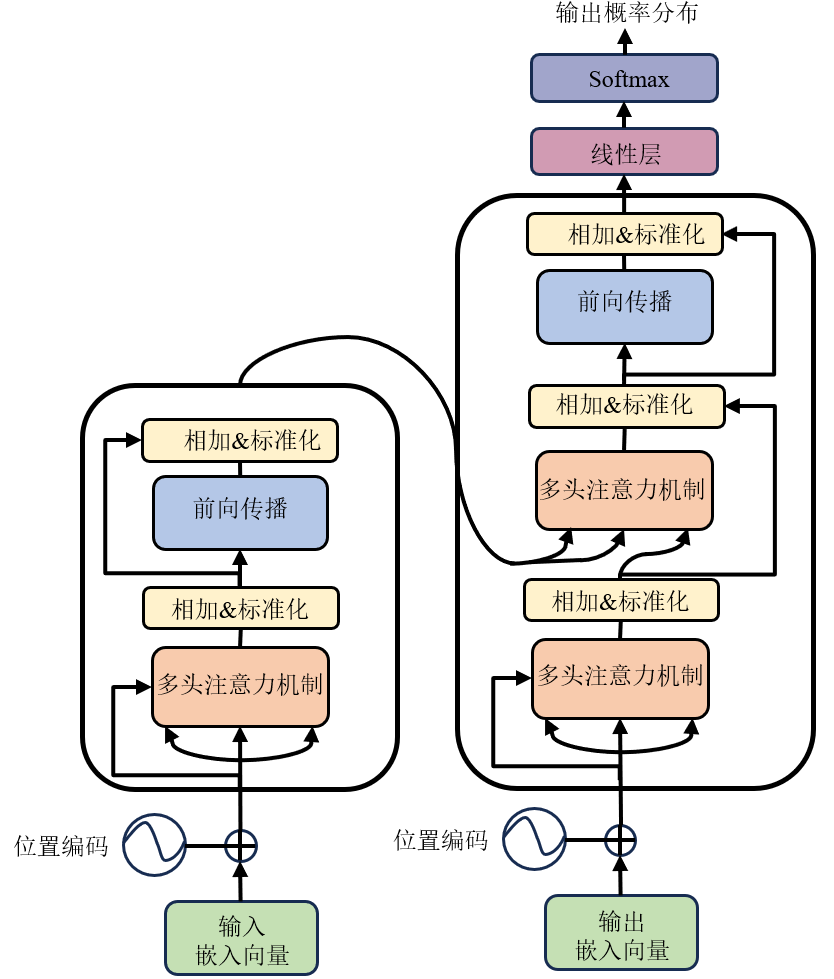
\includegraphics[scale=0.44]{transformer结构.png}
  \bicaption[transformer结构]{transformer结构}[]{ Transformer Structure}
  \label{fig:transformer}
\end{figure}
\begin{figure}[!htbp]
  \centering
  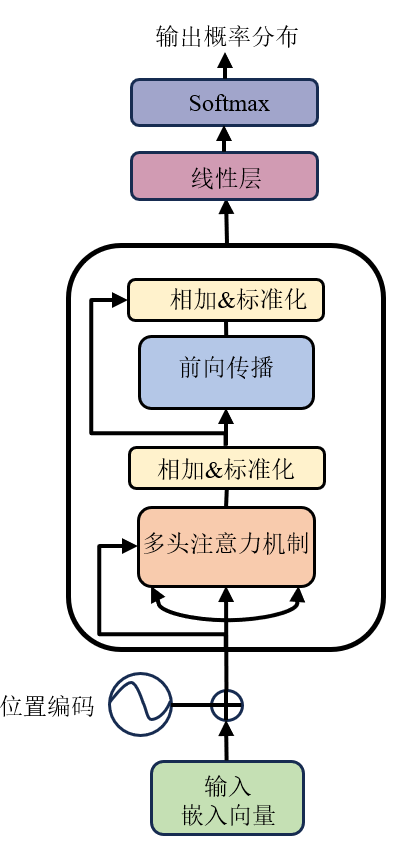
\includegraphics[scale=0.44]{encoderonly.png}
  \bicaption[encoder-only结构]{Encoder-only结构}[]{ Encoder-only Structure}
  \label{fig:encodel}
\end{figure}


\section{提示词学习}
提示词学习(Prompt Learning)是一种新的模型优化方法,通过设计输入格式或附加提示(prompts),使语言模型更好地理解任务意图并生成符合期望的输出。与传统微调(Fine-tuning)方法不同,提示词学习通常不需要修改模型参数,而是通过输入结构的调整激发模型内部的知识,从而完成特定任务。
\subsection{提示词学习理论基础}
提示词学习最早的雏形是由OpenAI在验证GPT-2模型能在无监督(zero-shot)的情况下学习语义与任务知识\cite{radfordLanguageModelsAre2019}。GPT-2模型在参数上达到了1542M,已经通过预训练学习了大量通用知识及理解能力,不需要再通过额外样本学习来完成任务,但仍需要通过一些方法令模型理解任务需求,输出符合预期的结果,如图\ref{fig:监督学习示意图}。图中以二分类情感分析任务为例,适当调整模型的输出层以适应任务后,通过大量的训练样本令模型学习语义知识并告诉模型面对不同的输入该对应什么结果,并将这种行为更新在模型参数中。因此,再次得到相似的输入时就可以得到正确输出。
\begin{figure}[!htbp]
  \centering
  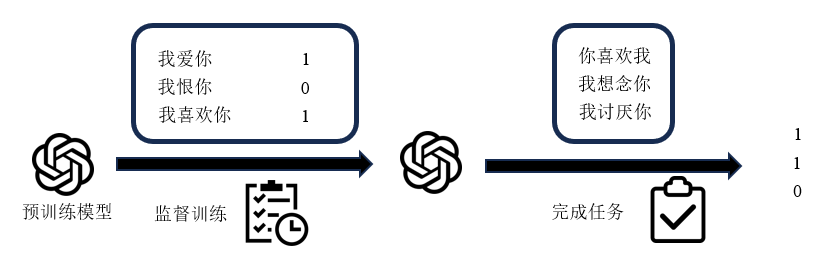
\includegraphics[scale=0.55]{监督训练示意图.png}
  \bicaption[监督学习示意图]{监督学习示意图}[Supervised Sraining]{Supervised Sraining}
  \label{fig:监督学习示意图}
\end{figure}

而面对大规模参数的预训练模型GPT-2时,研究人员认为通过大量的文本预训练以及百万参数量级的参数已经令模型具备足够的理解能力和通用知识,所以只需要简单的少样本(Few-shot)微调来使模型熟悉输入输出模式即可。但因为模型参数庞大,即使少量样本的训练也需要大量的运算资源,并且在特定任务下难以获取足够高质量样本,研究者们逐渐探索不需要特定任务数据下的零样本(zero-shot)方法来使预训练模型完成下游任务,即早期提示词学习的雏形。

在这种方法中,不对模型的参数进行更新而是对下游任务数据进行预处理,将文本嵌入进数据集中,通过文字的方式让模型理解任务的需求,同时规范化输出格式,如图\ref{fig: 零样本学习示意图}所示。
\begin{figure}[!htbp]
  \centering
  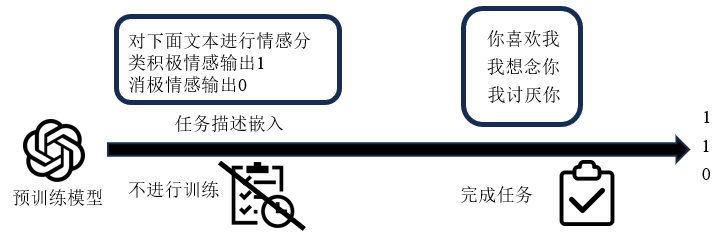
\includegraphics[scale=0.57]{零样本学习示意图.png}
  \bicaption[零样本学习示意图]{零样本学习示意图}[]{Zero-shot Learning}
  \label{fig: 零样本学习示意图}
\end{figure}

实验表明,这种只做文本嵌入不做特定训练框架的方法在多个自然语言处理任务中达到了最优结果,部分任务中远超基线模型。作者证明,具有足够容量的语言模型可以通过无监督学习执行多种任务,并在部分任务中达到或超过 SOTA (State of the Art)性能。这一发现为多任务学习和预训练语言模型的发展提供了重要的思路。即通过在数据中加入描述性文本来替代下游任务训练的无监督学习方法。

\subsection{提示词学习方法}

本节中介绍在实际应用中常用到的提示词学习方法,同时也是在检索增强系统中实际应用的方法,以便理解提示词在系统中的原理及意义。
少样本(Few-shot)学习是在零样本学习后提出的,根据零样本学习的研究成果,作者相信更大参数规模的模型配合上适量训练数据可以更进一步地提高模型在复杂下游任务上的表现,而训练数据也是作为提示词的形式输入给模型,不需要训练来更新参数就可以规范化模型的输出格式,如图\ref{fig: 少样本学习提示词样例}。图中展示了针对表格问答任务的输入输出样例。通过少量的样例就可以令模型理解任务,并且直接通过样例让模型理解任务需求的方式比直接通过语言描述任务需求效果更好更直观,还可以规范生成式模型的回答格式。以上方法为检索增强生成的核心原理,研究人员将之定义为离散提示词学习。
\begin{figure}[htbp]
  \centering
  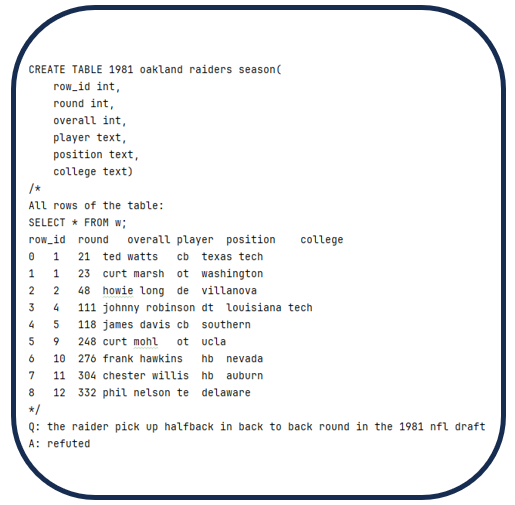
\includegraphics[scale=0.74]{少样本学习提示词样例.png}
  \bicaption[少样本学习提示词样例]{少样本学习提示词样例}[]{Few-Shot Learning Prompt Example}
  \label{fig: 少样本学习提示词样例}
\end{figure}


\section{神经网络模型压缩}
循环神经网络(Recurrent Neural Network,RNN)是一类在处理序列数据方面具有独特优势的神经网络,广泛应用于自然语言处理、时间序列分析等众多领域。其设计初衷是为了有效处理数据中的时间序列信息或序列依赖关系。从结构角度来看,RNN 区别于传统神经网络的核心特征是其具有反馈连接。在 RNN 的架构中,隐藏层既接收当前时刻输入层的信号,又会整合上一时刻隐藏层自身的输出信息。这一特性使得 RNN 能够在处理序列数据时,保留并利用先前时间步的信息,进而捕捉数据中的长期依赖关系。在$t$时刻的RNN单元可以表示为
\begin{equation}
  \label{eq:rnn}
  {h_t} = \varphi ({W_{xh}}{x_t} + {W_{hh}}{h_{t - 1}} + b)
\end{equation}
其中,$x_t$表示时刻t的输入向量,$h_{t-1}$是上一时刻$t-1$的隐藏层状态向量,$h_t$则为当前时刻的隐藏层状态向量;$W_{xh}$和$W_{hh}$分别是输入到隐藏层和隐藏层到隐藏层的权重矩阵,它们决定了不同输入对隐藏层状态的影响程度;$b$是偏置向量,用于增加模型的灵活性;$\varphi$代表激活函数,如常见的$sigmoid$函数、$tanh$ 函数等,其作用是对加权输入进行非线性变换,使模型能够学习到复杂的非线性关系。为方便与文章后续内容比较和理解循环神经网络与非线性动力学系统之间的联系将循环神经网络表示为公式\ref{eq:rnn2}。
\begin{equation}
  \label{eq:rnn2}
  {x_t} = f(A{x_{t - 1}} + B{u_t})
\end{equation}
其中$x_t$为当前t时刻的隐藏层状态,$A$为隐藏层到隐藏层的状态系数矩阵,$B$为输入到隐藏层的输入稀疏矩阵,$u_t$为当前时刻t的输入,$f()$表示激活函数。下面介绍动力学系统(dynamical system)及其非线性的内容及表达形式。

动力学系统是一门融合数学、物理学及工程学等多学科理论,专注于研究随时间演化的系统行为的学科领域。它通过建立数学模型,对系统状态随时间的变化规律进行精确刻画,揭示系统的内在动态特性,为众多科学与工程问题提供理论依据和解决方案。这里主要介绍离散非线性动力学系统,非线性动力学系统是动力学系统的一个重要分支,它聚焦于研究随时间演化的系统,且系统内各元素之间存在非线性相互作用关系。相较于线性系统,非线性动力学系统能够展现出更为丰富和复杂的行为,这些行为无法通过线性理论进行全面解释与预测从数学定义上看,非线性离散动力学系统通常由一组非线性差分方程来描述,如公式\ref{eq:discrete}。
\begin{equation}
  \label{eq:discrete}
  {x_k} = g({x_{k - 1}},{u_k},k)
\end{equation}
其中$x_k$为当前离散时刻$k$的状态,$u_k$为当前离散时刻$k$的输入,$g()$代表任意函数映射关系,当$g()$为非线性函数时,系统即为非线性离散动力学系统。通过表达系统内部各个状态于采样时间之间的映射关系来描述系统模型,并通过数学方法分析和处理系统。循环神经网络于动力学系统模型的具体关系将在第\ref{cha:第三章}章中详细介绍。

降维(Dimensionality Reduction)作为解决高维数据与复杂系统建模问题的核心思想,在神经网络模型压缩与动力学系统模型降阶中均占据重要地位。尽管二者分属机器学习与动力系统领域,但其方法论在降维思想上具有深刻的一致性,均通过对高维空间的结构化近似与稀疏化表示,实现模型复杂度的降低与计算效率的提升。神经网络模型压缩通过减少参数量与计算复杂度来优化模型性能,而动力学系统模型降阶则通过简化复杂微分方程描述的动态过程来降低数值求解的复杂度。二者的核心目标均是在保留关键特征的前提下,将高维空间映射至低维空间,从而实现高效建模与计算。

在神经网络模型压缩中,降维思想主要体现在参数剪枝\cite{liuFilterPruningQuantifying2023}、量化\cite{jacobQuantizationTrainingNeural2018}、知识蒸馏\cite{hintonDistillingKnowledgeNeural2015}以及低秩分解\cite{hanDeepCompressionCompressing2016}等方法中。参数剪枝通过移除冗余权重实现模型的稀疏化表示,其本质是对高维参数空间的降维操作,利用显著性准则(如权重幅值或梯度敏感度)识别并裁剪非关键连接,从而将稠密参数矩阵转化为稀疏矩阵。量化则通过将高精度浮点参数映射至低比特整数表示,实现参数空间的降维,极端情况下,二值化网络将权重约束为±1,将高维连续空间映射至低维离散空间。知识蒸馏利用教师网络的软标签指导轻量化学生网络的训练,本质上是将教师网络的高维特征空间压缩至学生网络的低维空间,通过提取教师网络的关键特征,学生网络能够在低维空间中近似原始模型的性能。低秩分解通过将权重矩阵分解为多个低秩矩阵的乘积,显著减少参数量,例如奇异值分解法(SVD)
\begin{equation}
  \label{eq:svd}
  W_n = U_n\Sigma_n {V_n^T}
\end{equation}
\begin{equation}
  \label{eq:Sigma}
{\Sigma_n} = \begin{array}{*{20}{c}}
  {{\sigma _1}}&0& \cdots &0\\
  0&{{\sigma _2}}& \cdots &0\\
   \vdots & \cdots & \cdots & \vdots \\
  0&0& \cdots &{{\sigma _n}}
  \end{array}
\end{equation}
其中$U_n$、$\Sigma_n$、$V_n$分别为权重矩阵$W_n$的左奇异值矩阵、奇异值矩阵与右奇异值矩阵,$\sigma_i$为矩阵$W_n$的奇异值,并按非递增顺序排列。通过保留主要奇异值与对应奇异值向量,实现权重矩阵的降维。将权重矩阵分解为奇异向量与奇异值的组合,或两个矩阵的乘积形式,从而减少参数量,
\begin{equation}
  \label{eq:lowrank}
  W_n \approx {\hat{U}_{n\times m}}{\hat{V}_{m\times n}^T}
\end{equation}
其中,$m(m<n)$为保留的奇异值个数,$\hat{U}$、$\hat{V}$分别为保留前$m$个向量的左奇异值矩阵和奇异值矩阵与右奇异值矩阵的乘积$\hat{V}=\Sigma_mV$,通过适当选择$m$,可以有效压缩参数量,保留主要奇异值以实现降维。这些方法在卷积神经网络中广泛应用,也是大模型的低秩近似轻量化微调(adapter)\cite{houlsbyParameterefficientTransferLearning2019}的主要理论方法,能够有效降低计算复杂度。

在动力学系统模型降阶中,降维思想则通过投影降阶、平衡截断、时间尺度分离以及非线性降维等技术实现。投影降阶通过基函数投影将高维状态空间映射至低维子空间,例如本征正交分解(POD)提取主成分构成降维基,将高维动力学系统嵌入到低维子空间中,从而保留系统的主要动态特征。平衡截断基于可控性与可观性Gram矩阵,剔除对输入-输出行为贡献微弱的状态变量,其本质是通过对状态空间的压缩,保留系统的主导动态行为。时间尺度分离通过奇异扰动理论将多速率系统的快慢变量分离,仅保留慢变子系统,利用系统动态特性的时间尺度差异,将高维动力学系统降维为低维慢变系统。

尽管神经网络模型压缩与动力学系统模型降阶在应用场景上存在差异,但二者的降维思想在数学本质与方法论上具有高度一致性。首先,二者均依赖于低维嵌入与稀疏表示的思想,模型压缩中的剪枝与量化可视为对参数空间的稀疏约束,而动力学降阶通过投影消除冗余状态变量,二者均利用稀疏性先验实现降维。其次,二者的优化目标具有同构性,均需最小化简化模型与原始模型的误差,例如知识蒸馏的损失函数与POD中的主成分保留均体现为对关键特征的提取与保留。此外,二者的方法论在某种程度上相互借鉴与融合,例如平衡截断中的Hankel范数优化思想可迁移至神经网络,通过分析权重矩阵的奇异值分布指导分层剪枝;而自编码器结构被引入非线性系统降阶,其编码器可视为数据驱动的POD基生成器,实现了从数据中自动提取低维特征。
然而,二者也存在一定差异。神经网络模型压缩侧重静态参数空间的优化,通常依赖数据驱动的方法;而动力学系统模型降阶则关注动态演化过程的近似,通常基于物理方程的先验知识。这种差异使得二者在具体实现上有所不同,但也为二者的协同提供了可能性。例如,在实时控制系统中,压缩后的轻量化网络可作为降阶模型的替代,实现嵌入式部署;而动力学降阶技术可为网络训练提供更高效的计算方法,提升训练效率。

\begin{table}[htb]
  \centering
  \begin{minipage}[t]{0.8\linewidth}
    \bicaption[模型压缩和模型降阶比较]{模型压缩和模型降阶比较}[Comparison of Model Compression and Model Reduction]{Comparison of Model Compression and Model Reduction}
    \label{tab:model-compression-reduction}
    \begin{tabularx}{\linewidth}{lXX}
      \toprule[1.5pt]
      {\heiti 参数} & {\heiti 模型压缩} & {\heiti 模型降阶} \\\midrule[1pt]
      定义 & 通过减少模型参数量与计算复杂度,保持性能 & 通过简化微分方程描述的动态过程,保留系统主要动态特征 \\
      数学本质 & 参数空间的稀疏约束与低维嵌入 & 状态空间的降维与简化 \\
      数据依赖性 & 依赖数据驱动 & 基于物理方程的先验知识 \\
      目的 & 平衡模型复杂度与精度,实现轻量化部署 & 保留系统主要动态行为,简化数值求解 \\
      主要技术 & 剪枝、量化、知识蒸馏、低秩分解 & 投影降阶、平衡截断、时间尺度分离、非线性降维 \\
      \bottomrule[1.5pt]
    \end{tabularx}
  \end{minipage}
\end{table}

神经网络模型压缩与动力学系统模型降阶在方法论上虽属于机器学习与动态系统领域,但其核心思想均以降维理论为基础,旨在通过低维嵌入与稀疏表示实现高维复杂系统的简化建模。二者在数学本质上具有显著共性:均需构造误差泛函以最小化简化模型与原始模型的特征偏差(如模型压缩的预测误差与降阶系统的动态响应误差),并依赖稀疏性约束(如参数剪枝与投影降阶)提取关键特征。然而,其差异主要体现在优化对象与应用层面:模型压缩聚焦于静态参数空间的轻量化(如权重矩阵的量化与低秩分解),依赖数据驱动方法优化边缘计算场景下的推理效率;模型降阶则针对动态演化过程(如微分方程状态变量的时间尺度分离),基于物理先验知识保留系统的可控性与可观性模态。此外,二者的理论基础亦存在差异——前者基于流形(flow)近似理论重构参数空间,后者则依托理论提取动态模态。尽管如此,两类方法在实时控制、嵌入式系统等交叉场景中展现出协同潜力,例如通过物理约束增强网络泛化性,或利用轻量化网络替代传统降阶模型,为跨领域的高效建模提供了新的理论框架。

循环神经网络(RNN)在连续提示词学习中的编码作用主要体现在其对时序动态特征的有效捕捉与上下文信息的渐进式建模。连续提示词\cite{liuPTuningV2Prompt2022}是在寻找最优离散提示词的基础上提出的,希望通过一段无实际含义但可训练的向量来代替离散的词向量,以实现最优的提示词效果。在连续提示词中最重要的是连续提示词向量的初始化嵌入,嵌入模型既要考虑编码的轻量性又要包含语序信息。RNN作为一种经典的序列模型,具有较好的时序建模能力,能够有效捕捉提示词序列中的长程依赖关系,成为了实现该功能的首选工具。
RNN通过其循环结构逐时间步处理连续提示词的序列输入,并通过隐藏状态传递历史信息。以长短期记忆网络(LSTM)为例,其门控机制(输入门、遗忘门、输出门)可自适应调节提示词序列中不同时间步的权重,从而区分关键提示与冗余噪声。例如,在对话生成任务中,LSTM可将用户输入的连续提示词(如上下文意图向量)编码为固定维度的隐藏状态,作为解码器的初始化上下文,确保生成文本的语义连贯性。此外,RNN通过迭代更新隐藏状态,实现对多层级提示特征的融合。在连续提示学习中,初始提示(如任务描述向量)与动态补充提示(如检索增强的上下文向量)可通过RNN的时序编码进行层次化整合。例如,在文本分类任务中,双向GRU(门控循环单元)可将任务相关的连续提示词与输入文本的嵌入向量按时间顺序融合,生成上下文敏感的特征表示,提升模型对复杂语义边界的判别能力。

相比于Transformer等自注意力模型,RNN的计算复杂度与序列长度呈线性关系,更适合资源受限场景下的连续提示学习。通过参数共享与增量式处理,RNN能够以较低内存开销支持实时动态提示调整。在低资源机器翻译任务中,基于LSTM的连续提示编码器可将推理延迟降低,同时保持良好的效果。然而,RNN在长程依赖建模能力上存在局限性,未来研究可通过引入记忆增强机制或混合架构(RNN-Transformer协同编码)提升对长提示序列的建模效果。此外,基于可微分结构的动态提示剪枝技术可进一步优化RNN编码效率,实现关键提示特征的精准提取。RNN通过其固有的时序建模能力,在连续提示词学习中实现了对动态提示特征的渐进式编码与上下文感知融合,为轻量化、实时性要求高的任务提供了高效解决方案,未来结合记忆增强与混合架构的设计有望突破其长序列建模瓶颈,推动提示学习的进一步发展。
\section{检索增强生成}
检索增强生成(Retrieval-Augmented Generation, RAG)\cite{karpukhinDensePassageRetrieval2020,izacardFewshotLearningRetrieval2022,yaoEditingLargeLanguage2023,fengTrendsIntegrationKnowledge2023,xuRetrievalMeetsLong2024,balaguerRAGVsFinetuning2024}是一种将外部知识库动态集成到生成模型中的技术方法,其核心目标是通过引入结构化检索机制增强生成内容的准确性、逻辑性与事实一致性。与传统端到端生成模型依赖内部参数化知识不同,RAG系统通过“检索-推理-生成”的协同机制,将生成过程与外部知识库实时交互,有效解决了模型幻觉(Hallucination)与长尾知识覆盖不足等问题。该技术的实现依赖于三个核心组件:检索器(Retriever)、向量知识库(Vector Knowledge Base)与智能协调体(Agent),并通过思维链(Chain of Thought, CoT)的渐进式推理框架实现复杂任务的分解与求解。

在科学问答任务中,传统模型在处理跨学科知识的复杂问题时,常因模型参数偏差导致错误传播,影响答案准确性。而结合思维链(CoT)机制的RAG系统则有效克服了这一局限。
当用户提出涉及多学科知识交叉的复杂问题时,RAG系统首先通过检索器从大规模向量知识库中精准提取与问题高度相关的文档片段。这些片段可能来自不同学科领域,为后续推理提供了知识支撑。接着,系统基于这些检索到的内容,构建出多步推理路径的上下文。这一过程模拟了人类专家在面对复杂问题时的渐进式思维模式,将不同来源的知识有机整合,形成连贯的推理链条。
最后,系统依据构建好的推理链上下文,生成逻辑连贯、内容完整的答案。整个过程通过引入外部知识约束,有效降低了传统模型因参数偏差导致的错误传播风险。

检索器作为连接生成模块与知识库的核心枢纽,其性能直接决定了知识检索的精度与效率。当前主流方法主要分为稀疏检索与密集检索两类:稀疏检索器,基于词频统计构建查询与文档的匹配关系,具有计算效率高的优势,但对语义相似性的捕捉能力有限。典型代表为BM25\cite{robertsonProbabilisticRelevanceFramework2009}算法,通过将目标文本$Query$分词为单个token $q_i$后,再分别计算$q_i$对于某一文本$d$的相似度加权和,如公式\ref{eq:bm25}
\begin{equation}
  \label{eq:bm25}
  \text{score}(q, d) = \sum_{i} W_i \cdot R(q_i, d)
  \end{equation}
其中$W_i$为$q_i$的权重,$R(q_i, d)$为$q_i$与$d$的相似度函数。相似度函数$R()$一般使用余弦相似度计算。
\begin{equation}
  \text{similarity} = \cos(\theta) = \frac{\mathbf{A} \cdot \mathbf{B}}{\|\mathbf{A}\|\|\mathbf{B}\|} = \frac{\sum_{i=1}^{n} a_i \times b_i}{\sqrt{\sum_{i=1}^{n} (a_i)^2} \times \sqrt{\sum_{i=1}^{n} (b_i)^2}}.
  \end{equation}
其中$\mathbf{A}$、$\mathbf{B}$代表需要计算相似度的两个高维向量,$a_i$、$b_i$为对应向量的每个维度上的分量。
密集检索器(如基于BERT、DPR的深度模型)通过神经网络将文本映射为高维稠密向量,利用向量空间相似度实现语义级检索,能够识别查询与文档间的隐含关联,但需依赖大规模训练数据与计算资源。为平衡效率与精度,混合检索架构(如ColBERT模型)通过上下文感知的多向量表示方法,对文档不同片段进行细粒度匹配,在长文本检索场景中表现出显著优势。与此同时,向量知识库的构建与管理面临数据标准化、嵌入编码优化与动态更新等挑战。当前研究通过分块策略(Chunking)与实体链接技术实现非结构化文本的预处理,采用Sentence-BERT等预训练模型生成文档嵌入,并借助FAISS等最邻近算法(Approximate Nearest Neighbor,ANN)等近似最近邻算法建立高效索引。

智能体(Agent)作为RAG系统的控制中枢,负责动态调控检索与生成模块的交互策略。其核心功能包括检索触发决策、多轮检索优化与结果融合策略。例如,当输入问题涉及常识性知识时,Agent可直接调用模型内部参数化知识生成答案;而对于专业性较强的查询,则触发外部检索流程获取补充信息。在生成过程中,若检测到中间推理结果的置信度不足,Agent可发起多轮检索以迭代补充证据。为实现多源检索结果的融合,系统常采用注意力机制对相关片段进行加权聚合,或通过最大内积搜索(MIPS)筛选最相关段落。在技术实现上,智能体多基于强化学习框架构建,通过策略梯度方法优化决策过程,其目标函数同时考虑答案准确性、检索效率与资源消耗等多维度指标。

尽管RAG技术在知识密集型任务中展现出巨大潜力,其实际应用仍面临多重挑战。首先,密集检索与多轮推理导致的系统延迟问题亟待解决,轻量级检索架构(如基于知识蒸馏的检索器压缩)与硬件加速技术成为研究热点。其次,静态向量知识库难以适应动态演化的外部知识环境,如何实现流式数据下的在线嵌入更新与知识修正仍需深入探索。此外,当前RAG系统主要面向文本模态,如何融合图像、视频等多模态知识以支持跨媒体推理成为重要发展方向。未来研究可聚焦于构建端到端可微的联合训练框架,通过检索与生成模块的参数共享提升系统整体效率;开发基于因果推理的检索验证机制,增强生成结果的可解释性;同时拓展RAG在科学发现、法律咨询等垂直领域的应用边界,推动知识驱动型人工智能的实用化进程。
\section{本章小结}
本章系统阐述了基于大模型的智能反馈交互系统的核心理论基础,为后续系统的设计提供了理论支撑与方法论框架。首先,通过分析生成式自回归神经网络(如GPT、LLaMA等)的架构特性,揭示了其通过自回归机制实现序列生成的内在原理,并重点讨论了Transformer模型中的注意力机制与分词器对语义建模的关键作用。其次,从零样本学习到少样本学习的演进路径出发,剖析了提示词学习(Prompt Learning)通过输入任务指令与非参数化知识提高模型下游任务表现的核心逻辑,为检索增强生成(RAG)系统的动态知识整合提供了方法论基础。

在模型压缩理论部分,通过对比神经网络模型压缩与动力学系统模型降阶的数学本质,提出二者均以降维思想为核心,分别通过参数稀疏化与状态空间投影实现高效压缩。特别地,针对循环神经网络(RNN)在连续提示词编码中的文本嵌入能力,分析了其在轻量化推理中的独特优势,为后续基于本征正交分解的模型压缩方法提供了理论依据。  

最后,聚焦检索增强生成(RAG)技术,系统阐释了其“检索-推理-生成”协同的工作机理,强调了检索器、向量知识库与智能协调体的协同优化策略。通过对比稀疏检索与密集检索的技术差异,以及知识库动态更新的实现路径,揭示了RAG系统在知识密集型任务中的核心价值。本章内容不仅为后续章节的模型压缩算法设计、表格推理框架构建及反馈系统实现奠定了理论基础,更通过跨学科视角(如动力学系统与深度学习的融合)为轻量化智能系统的开发提供了创新性研究方向。



% !Mode:: "TeX:UTF-8"
\chapter{循环神经网络的轻量化压缩}
\label{cha:第三章}
本章节提出了一种基于动力学模型降阶方法——本征正交分解法的循环神经网络模型压缩方法。首先,介绍了循环神经网络及其变体长短期记忆网络的基本结构及其动力学模型。然后,详细介绍了本征正交分解法的原理和算法。最后,将本征正交分解法应用于循环神经网络模型压缩。实验结果表明,本征正交分解法可以有效地压缩循环神经网络模型,同时保持模型的预测性能。
\section{问题描述}
尽管以Transformer为核心架构的大语言模型凭借其全局注意力机制与并行化计算优势,在自然语言处理领域占据主导地位,但循环神经网络(Recurrent Neural Network, RNN)在连续提示词编码场景中仍展现出独特的应用价值与轻量化潜力\cite{liuGPTUnderstandsToo2023,liuPTuningV2Prompt2022}。相较于Transformer模型依赖自注意力机制构建长程依赖所导致的高计算复杂度,RNN通过参数共享时序建模特性,能够以更低的内存开销实现连续提示词编码。这一特性使其在资源受限场景中具有显著优势。进一步地,RNN的循环结构适配轻量化压缩需求。通过动力学系统视角下的模型降阶方法,可对RNN隐藏状态进行低维投影,在保留时序动态特征的前提下实现参数的高效压缩。

% 例如,在连续提示词学习中,双向门控循环单元(BiGRU)可通过门控机制自适应调节多层级提示(如任务描述向量与检索增强上下文)的融合权重,生成上下文敏感的低维向量表示,而无需依赖Transformer的高维多头注意力计算。
伴随着神经网络的发展,出现了更多新的研究视角。有论文将神经网络看作常微分方程或动力学系统\cite{chenNeuralOrdinaryDifferential2019}。在以往的许多工作中,循环神经网络都被表示成常微分方程\cite{rubanovaLatentODEsIrregularlySampled,mozerDiscreteEventContinuous2017},并使用动力学系统中的方法处理它。受前人工作启发,文中提出一种动力学系统模型降阶方法来降低长短期记忆网络模型隐藏层状态的维度,该方法可以压缩权重矩阵并减少计算量。

面对神经网络模型的发展,为了实现更好的性能而模型参数越来越大,于是面临着设备存储资源有限而部署困难的问题\cite{dengModelCompressionHardware2020},同时也面对边缘设备无法支持庞大的计算量所需要的能源问题\cite{hanDeepCompressionCompressing2016}。需要能够同时压缩模型参数和推理计算量的模型压缩方法来解决神经网络的工程实践问题。循环神经网络与卷积神经网络不同,循环神经网络的前向传播通常由时间序列决定并且每一时间步上的隐藏层状态使用相同的权重矩阵。隐藏层状态包含着大量的特征信息,其节点数量决定了循环神经网络的权重矩阵和计算量的大小。隐藏层状态的维度是一种超参数,往往无法定义最合适的维度,在大多数情况下,设置的隐藏层维度会高于实际编码特征所需要的维度,这就造成了参数的冗余。所以希望提出一种方法能够将隐藏层的维度压缩至合适的大小,则可以减少参数量和计算量。因此,提出了一种基于本征正交分解的模型压缩方法,该方法的原理是用低维向量近似原始的高维向量。
实验应用了一个两层长短期记忆网络去完成在固定时间序列的分类问题,并使用本征正交分解的方法可以在精度损失很少的情况下,将其压缩。

% 在自然语言处理领域,Transformer大语言模型凭借全局注意力机制与并行化计算优势占据主导地位,但循环神经网络(RNN)在连续提示词编码场景中仍具独特价值与轻量化潜力\cite{liuGPTUnderstandsToo2023,liuPTuningV2Prompt2022}。与Transformer依赖自注意力机制构建长程依赖导致高计算复杂度不同,RNN通过参数共享时序建模,能以更低内存开销实现连续提示词编码,使其在资源受限场景(如边缘计算设备或实时交互系统)中更具优势。例如,双向门控循环单元(BiGRU)可通过门控机制自适应调节多层级提示的融合权重,生成上下文敏感的低维向量表示,无需依赖Transformer的高维多头注意力计算。此外,RNN的循环结构天然适配轻量化压缩需求,通过动力学系统视角下的模型降阶方法(如本征正交分解),可对RNN隐藏状态进行低维投影,在保留时序动态特征的前提下实现参数的高效压缩。

% 随着神经网络的发展,出现了多种研究视角,有论文将其视为常微分方程或动力学系统\cite{chenNeuralOrdinaryDifferential2019},许多工作中循环神经网络被表示为常微分方程\cite{rubanovaLatentODEsIrregularlySampled,mozerDiscreteEventContinuous2017}并使用动力学系统方法处理。受此启发,本文提出一种动力学系统模型降阶方法来降低长短期记忆网络模型隐藏层状态的维度,以压缩权重矩阵并减少计算量。然而,神经网络模型为追求更好性能导致参数规模越来越大,面临设备存储资源有限、部署困难的问题\cite{dengModelCompressionHardware2020},同时边缘设备也难以支持庞大计算量所需的能源\cite{hanDeepCompressionCompressing2016},因此需要能同时压缩模型参数和推理计算量的模型压缩方法来解决工程实践问题。

% 循环神经网络与卷积神经网络不同,其前向传播由时间序列决定,且每一时间步上的隐藏层状态使用相同的权重矩阵。隐藏层状态包含大量特征信息,其节点数量决定了循环神经网络的权重矩阵和计算量的大小。隐藏层状态的维度是一种超参数,往往难以定义最合适的维度,大多数情况下设置的隐藏层维度会高于实际编码特征所需要的维度,造成参数冗余。因此,本文提出一种基于本征正交分解的模型压缩方法,其原理是用低维向量近似原始的高维向量。实验中,应用了一个两层长短期记忆网络完成固定时间序列的分类任务,并使用本征正交分解的方法,在几乎不损失精度的情况下成功将其压缩。

\section{本征正交分解法}
本征正交分解法\cite{nomuraStructureInhomogeneousTurbulence1993}作为一种基于数据驱动的降维方法,其核心思想是通过提取高维动力学系统状态空间中的主导信息,构建低维子空间以近似原始系统的方法。该方法能够通过一组正交基降低非线性动力学系统模型的维度,是一种常见的模型降阶方法,其在流体力学、结构动力学等领域已得到广泛应用。在文中被引入神经网络模型压缩领域,为解决循环神经网络(RNN)参数量冗余与计算效率问题提供了新思路。
本征正交分解法(POD)的核心思想是将$k$个样本点的$n$维数据,投影到$m$维,即$n$维的数据可以被$m$维的数据近似,并且$m<<n$。假设有$k$个采样数据

\begin{equation}
  \label{eq:1}
X = \{ {x_1},{x_2},...,{x_k}\}  \in {R^{n \times k}}
\end{equation}
通过奇异值分解法(Singular Value Decomposition, SVD)计算样本数据 的一组正交基向量$\{ {\phi _i}\} _{i = 1}^n$,使对于每一个${x_i} \in {R^n},i \in [1,k]$都能够被表示为正交基向量的线性组合
\begin{equation}
  \label{eq:2}
{x_i} = {y_1}{\phi _1} + {y_2}{\phi _2} +  \cdots  + {y_n}{\phi _n},{\rm{ }}{y_i} \in R
\end{equation}
由于在SVD计算过程中基向量$\{ {\phi _i}\} _{i = 1}^n$按照能代表的信息量递减排序,所以可以用信息密度最高的前$m$项来近似原始样本数据,即
\begin{equation}
  \label{eq:3}
  {x_m} = {y_1}{\phi _1} + {y_2}{\phi _2} +  \cdots  + {y_m}{\phi _m}
\end{equation}
记作${x_m} = \phi {{\bf{y}}_m},{{\bf{y}}_m} \in {R^m}$。将原始数据和近似数据之间的误差定义为
\begin{equation}
  \label{eq:4}
{\varepsilon ^2} = \sum\limits_{i = 1}^m {\left\| {{x_i} - {x_{i(m)}}} \right\|_2^2}  = \sum\limits_{j = m + 1}^n {\phi _j^T} X{X^T}{\phi _j}
\end{equation}
其中$X = \{ {x_1},{x_2},...,{x_k}\} $。通过构建拉格朗日方程最小化误差,得到最小误差下的一组正交基向量$\{ {\phi _i}\} _{i = 1}^n$为采样数据点${X^T}$的右奇异值矩阵$V$ \cite{chatterjeeIntroductionProperOrthogonal2000}。误差定义为最后$n-m$项奇异值的平方和。
\begin{equation}
\label{eq:5}
  {X^T} = U\sum {V^T}
\end{equation}
其中$X$为采样数据点$\{ {x_1},{x_2},...,{x_k}\}  \in {R^{n \times k}}$,$\sum $为降序排列的奇异值对角矩阵,$U$是左奇异值矩阵,$V$是右奇异值矩阵并且满足
\begin{equation}
\label{eq:6}
UV = I
\end{equation}
其中$I$为单位矩阵。下面介绍POD的基本降阶过程。
对于以下非线性离散动力学系统,
\begin{equation}
\label{eq:7}
\left\{ \begin{array}{l}
  {x_{t + 1}} = f({x_t},{u_t}),\\
  {y_t} = g({x_t},{u_t}),
  \end{array} \right.
\end{equation}
其中函数$f( \cdot ) \in {R^n}$和函数$g( \cdot ) \in {R^o}$为非线性函数,${u_t} \in {R^i}$为系统输入,${y_t} \in {R^o}$为系统输出。取一定连续时间内的系统状态
\begin{equation}
\label{eq:8}
X = \{ {x_1},{x_2},...,{x_k}\}  \in {R^{n \times k}}
\end{equation}
为需要降阶近似的数据。设矩阵$V,W \in {R^{n \times m}}$$(m<n)$满足
\begin{equation}
\label{eq:9}
{V^T}V = {I_m}  
\end{equation}
根据上文方法得到$k$维基向量矩阵
\begin{equation}
\label{eq:10}
{\varPhi  _k} = [{\varphi _1},{\varphi _2},...,{\varphi _k}]
\end{equation}
令
\begin{equation}
\label{eq:11}
V = W = {\phi _k} \in {{\bf{R}}^{n \times k}}
\end{equation}
则${\hat x_t} = \phi _k^T{x_t}$为${x_t}$到$\phi _k^T$所在空间上的投影。$W$由采样数据 的右奇异值矩阵前$m$项组成。系统\ref{eq:7}降阶后的系统为,
\begin{equation}
\label{eq:12} 
\left\{ \begin{array}{l}
  {x_{t + 1}} = {W^T}f(V{{\hat x}_t},{u_t}),\\
  {y_t} = g(V{{\hat x}_t},{u_t}),
  \end{array} \right.
\end{equation}
其中${\hat x_t} \in {R^m}$。可以通过投影矩阵$W$, $V$得到降阶系统。
\section{动态循环神经网络}
循环神经网络作为时间序列建模常用模型,在不同采样时间下具有连续变化的状态,每个采样时间下的结果取决于上一个采样的结果和当前的输出,并且每次计算的系数矩阵和函数相同,这点与动力学系统类似,且由于激活函数的存在,可以将循环神经网络视作非线性动力学系统。为验证循环神经网络与动力学系统的相似性,分别使用循环神经网络和动力学系统模型简单对一个时间序列进行建模,并比较结果。
实验使用RNN模型拟合一个正弦函数映射到余弦函数的序列模型。自定义一个32节点单层循环神经网络,使用正弦函数作为输入,余弦函数作为标签训练输出,采样频率为1/0.0625π HZ。将得到训练后的RNN模型参数作为动力学系统的微分方程形式,将RNN网络表示为
\begin{equation}
\label{eq:13}
{h_{t + 1}} = f({h_t} + {x_t})
\end{equation}
其中$h_t$代表$t$时刻隐藏层状态,$x_t$代表$t$时刻输入,$f$为RNN结构,由RNN训练后的模型参数决定。将公式\ref{eq:13}等式两边同时减去$h_t$得到
\begin{equation}
\label{eq:14}
{h_{t + 1}} - {h_t} = f({h_t} + {x_t}) - {h_t}
\end{equation}
将公式\ref{eq:14}连续化为微分方程形式得到
\begin{equation}
\label{eq:15}
  {\dot h_t} = \frac{1}{{\Delta t}}(f({h_t} + {x_t}) - {h_t})
\end{equation}
通过这种变换得到了 的微分方程,使用积分器得到后续状态,即ODE-RNN的前向传播,根据数据得到图像, 实验结果如图\ref{fig:函数拟合结果}所示。
\begin{figure}[!htbp]
  \centering
  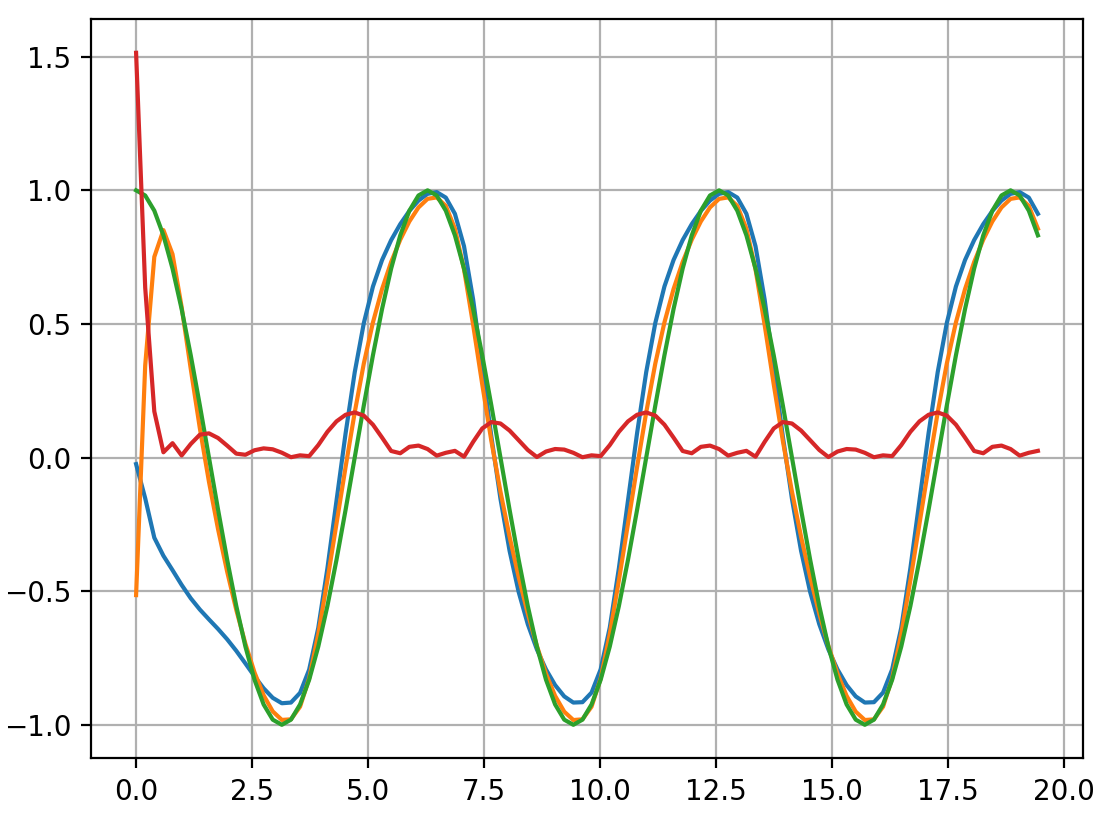
\includegraphics[width=0.7\textwidth]{函数拟合结果.png}
  \bicaption{函数拟合结果}{Comparison of Cosine Function Modeling}
  \label{fig:函数拟合结果}
\end{figure}
绿色波形为标准余弦信号,橙色波形为动力学系统建模。实验结果表明将原本训练好的RNN参数带入到微分方程中能够完成功能,表明了在参数相同时动力学系统与神经网络的一致性。
尽管传统循环神经网络在时间序列建模中可通过离散化常微分方程形式表征
其动力学特性,但其在长期依赖任务(如长程时间序列分类)中表现受限。这一局限性主要源于梯度消失/爆炸等问题,导致网络难以有效捕捉跨时间步的时序关联性。
为解决此问题,长短期记忆网络(Long Short-Term Memory, LSTM)\cite{hochreiterLongShorttermMemory1997}通过引入门控机制(输入门、遗忘门、输出门)重构了隐藏状态的动态演化过程。具体而言,遗忘门通过可学习的权重系数调节历史信息的保留比例,而输入门则动态控制当前输入的融合强度,从而实现对长期依赖的显式建模。实验表明,门控机制对复杂时序模式捕获的有效性。
然而,LSTM的高参数维度(如隐藏层维度为128时参数量达70k)导致其在资源受限场景下的部署面临挑战。为此,本征正交分解(Proper Orthogonal Decomposition, POD)方法被引入模型压缩领域。通过提取LSTM隐藏状态空间中的主导信息,POD将原始高维状态投影至低维子空间,并重构动力学方程。这一方法通过保留关键信息,在轻量化与性能间实现了高效平衡。

对于一个多层长短期记忆网络(如图\ref{fig:LSTM}所示),
\begin{figure}[hbp]
  \centering
  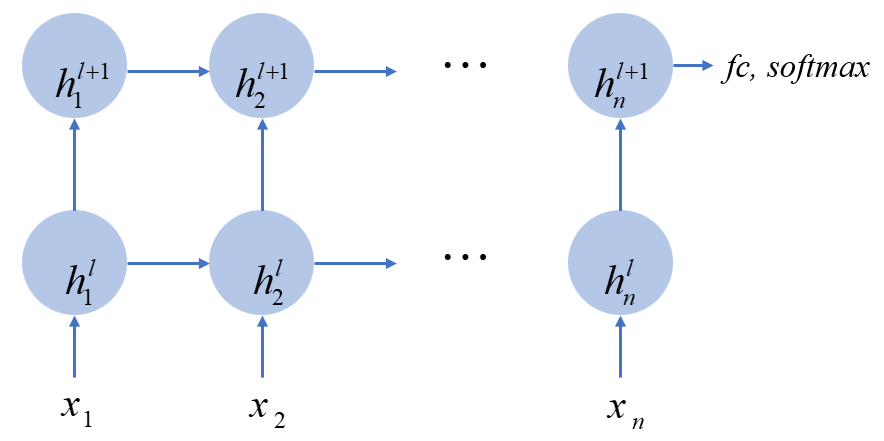
\includegraphics[width=0.7\textwidth]{多层长短期记忆网络结构.png}
  \bicaption{多层长短期记忆网络结构}{ the Multilayer LSTM Structure}
  \label{fig:LSTM}
\end{figure}
可以被表示为以下非线性的离散动力学系统,
\begin{equation}
\label{eq:16}
h_{t + 1}^l = f(W_i^l{x_{t + 1}} + W_h^lh_t^l + {b^l})
\end{equation}
\begin{equation}
\label{eq:17}
h_{t + 1}^{l + 1} = f(W_i^{l + 1}h_{t + 1}^l + W_h^{l + 1}h_t^{l + 1} + {b^{l + 1}})
\end{equation}
其中$f( \cdot )$为长短期记忆单元,$W_i^l \in {R^{n \times i}}$为第$l$层的输入矩阵,$W_h^l \in {R^{n \times n}}$是第$l$层的隐藏层矩阵,${b^l} \in {R^n}$为第$l$层的偏置。通过本征正交分解法计算投影矩阵$V \in {R^{n \times m}}$($m$是隐藏层 的新维度),并用其线性组合$h = V\hat h$来近似$h$。$\hat h \in {R^m}$为新隐藏层的系数矩阵,用$V\hat h$替换等式\ref{eq:16}和等式\ref{eq:17}中的$h$,得到
\begin{equation}
  \label{eq:18}
  \hat h_{t + 1}^l = {U^l}f(W_i^l{x_{t + 1}} + W_h^l{V^l}\hat h_t^l + {b^l})
  \end{equation}
\begin{equation}
  \label{eq:19}
  \hat h_{t + 1}^{l + 1} = {U^{l + 1}}f(W_i^{l + 1}{V^l}\hat h_{t + 1}^l + W_h^{l + 1}{V^{l + 1}}\hat h_t^{l + 1} + {b^{l + 1}})
  \end{equation}
其中$U^l$为$V^l$的转置,满足$U=V^T$。新的模型可以被表示为
\begin{equation}
  \label{eq:18}
  \hat h_{t + 1}^l = {U^l}f(W_i^l{x_{t + 1}} + \hat W_{\hat h}^l\hat h_t^l + {b^l})
  \end{equation}
\begin{equation}
  \label{eq:19}
  \hat h_{t + 1}^{l + 1} = {U^{l + 1}}f(\hat W_i^{l + 1}\hat h_{t + 1}^l + \hat W_{\hat h}^{l + 1}\hat h_t^{l + 1} + {b^{l + 1}})
  \end{equation}
其中$\hat W_{\hat h}^l = W_h^l{V^l} \in {R^{n \times m}}$,$\hat W_i^{l + 1} = W_i^{l + 1}{V^l} \in {R^{n \times m}}$,$\hat W_{\hat h}^{l + 1} = W_h^{l + 1}{V^{l + 1}} \in {R^{n \times m}}$, $\hat h \in {R^m}$ 。

通过将隐藏状态投影到较低的状态,可以获得具有较少参数和隐藏状态的模型,如图\ref{fig:原始模型和压缩模型的结构}所示,直观地展示新模型与原始模型在参数和隐藏层维度上的维度差异。其中$i$,$f$,$c$,$o$分别代表输入门、遗忘门、控制们和输出门。$W$,$V^T$分别代表每个们的权重矩阵和投影矩阵,$b$代表偏执,$h_t$,$c_t$,$o_t$分别代表$t$时刻的隐藏层状态、控制状态和输出状态。符号$\hat  \cdot $标志压缩后的模型参数。

在长短期记忆网络模型中,每层网络的隐藏层都有四个门控系数矩阵和输入系数矩阵。
降低以上矩阵的维度来达到压缩的目的。

\begin{figure}[!htbp]
  \centering
  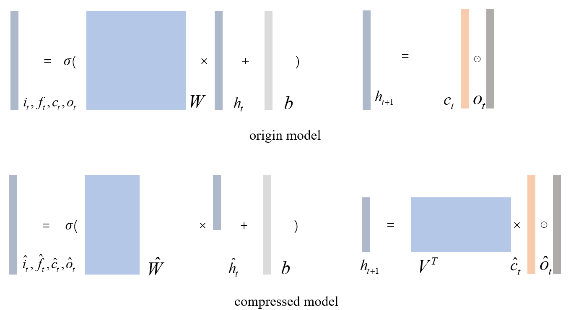
\includegraphics[width=0.74\textwidth]{原始模型和压缩模型的结构.png}
  \bicaption{原始模型和压缩模型的结构}{The Structure of the Original Model and Compressed Model.}
  \label{fig:原始模型和压缩模型的结构}
\end{figure}
\section{实验设置}
实验使用一个两层,隐藏层维度为72的长短期记忆网络来验证该方法的有效性。
实验使用UCI-HAR数据集\cite{anguitaHumanActivityRecognition2012}验证方法效果。UCI-HAR数据集是一个广泛应用于人类活动识别领域的公开数据集,它通过在智能手机上搭载的传感器收集了30名志愿者在进行六种日常活动(步行、上楼梯、下楼梯、静坐、站立和平躺)时产生的动态数据。这些数据由加速度计和陀螺仪以50Hz的频率采集得到,涵盖了三轴的线性加速度和角速度信息。在数据预处理阶段,研究者们通过噪声滤波器和巴特沃斯低通滤波器对原始数据进行了清洗和分离,以区分重力和身体运动分量,并计算了包括时域和频域在内的561个特征向量。数据集被分为训练集和测试集,其中训练集包含了21名志愿者的数据,而测试集则包含了剩余9名志愿者的数据。数据集有6个分类结果,9个特征和128次时间序列采样。综上,确定模型的输入系数矩阵、输出系数矩阵和时间长度,一共包含60k参数。
首先在Pytorch框架下利用标准LSTMcell和Adam优化器训练原始大小的模型。得到在测试集上准确度为85\%的基线模型。再利用本征正交分解压缩的模型与之进行对比。
将网络看作一个关于输出为$x$,隐藏层为$h$的非线性系统。全连接层作为输出函数。
\begin{equation}
  \label{eq:20}
\left\{ \begin{array}{l}
  {h_{t + 1}} = f({x_t},{u_t}),\\
  {y_t} = fc({h_t}),
  \end{array} \right.
\end{equation}
其中$fc( \cdot )$为全连接层。模型的隐藏层$h_i^l$可以被看作是非线性系统的状态变量,记作$\{ h_1^l,h_2^l,...,h_n^l\}$。模型的每一层隐藏层都分别用一组正交基$V$表示。正交基$V$可由算法\ref{algo:projecting_matrix}计算。
\begin{algorithm}[!htbp]
  \caption{得到投影矩阵}
  \label{algo:projecting_matrix}
  \DontPrintSemicolon
  \SetKwInOut{Input}{输入}
  \SetKwInOut{Output}{输出}
  \SetKwFunction{LSTM}{LSTM}
  \SetKwFunction{Average}{average}
  \SetKwFunction{SVD}{svd}
  
  \Input{1 批次训练数据,长短期记忆网络模型}
  \Output{投影矩阵 $V$}
  
  \vspace{5pt}
  
  $\{h_1, h_2, ..., h_n\} = \LSTM(\text{dataset})$\;
  $\mathbf{H} = \Average(\sum_{i=1}^{\text{batch\_size}} \{h_1, h_2, ..., h_n\})$\;
  $U \Sigma V' = \SVD(\mathbf{H}')$\;
  $V = V[:, 1:m]$\;
  
\end{algorithm}

在本研究中,为提升矩阵$V$的泛化性能,引入平均值函数 $average(\cdot)$,通过对所有输入数据进行平均值计算,降低模型的过拟合风险,增强其对未知数据的泛化能力。奇异值分解(SVD)函数$svd(\cdot)$被应用于计算矩阵$V$,通过分解矩阵揭示其内在特征,降低维度,去除冗余信息,提高模型的计算效率和泛化能力。投影矩阵$V$可以从模型的任意状态序列中导出,为模型架构提供高度灵活性,但不同的$V$矩阵选择可能导致不同程度的精度损失,需权衡泛化能力和精度。计算平均值的方法在数据量较大的情况下,能够更有效地整合信息,提升模型的泛化能力,通过在更大的数据集 的隐藏层状态$h$上计算平均值,捕捉数据分布特征,减少估计偏差。尽管利用复数数据在优化矩阵$V$方面取得了显著成效,但理论上还存在其他潜在的方法,如正则化技术或深度学习方法,可能进一步提升矩阵$V$的性能。
\section{结果分析}
原始自定义长短期记忆网络作为基线模型,利用基于本征正交分解的模型压缩方法将模型压缩至不同压缩比,利用不同隐藏层节点数量区分压缩模型,验来证模型性能和方法的科学性。
\begin{table}[htb]
  \centering
  \begin{minipage}[t]{0.8\linewidth}
    \bicaption[不同压缩维度下结果]{不同压缩维度下结果}[The Result in Different Compression Dimensions]{The Result in Different Compression Dimensions}
    \label{tab:compression-results}
    \begin{tabularx}{\linewidth}{lXXXX}
      \toprule[1.5pt]
      {\heiti 模型} & {\heiti 参数压缩比} & {\heiti 参数量} & {\heiti 计算量压缩比}  & {\heiti 准确率} \\\midrule[1pt]
      基线 & - & 9.5M & - &  85.0\% \\
      HNN=72 & - & - & - &  85.0\% \\
      HNN=64 & 93.5\% & 7.5M & 79.2\% &  84.6\% \\
      HNN=54 & 73.7\% & 5.4M & 56.7\% &  81.8\% \\
      HNN=46 & 52.6\% & 3.9M & 41.3\% &  81.8\% \\
      HNN=36 & 34.4\% & 2.4M & 25.6\% &  80.0\% \\
      HNN=28 & 22.7\% & 1.5M & 15.7\% &  66.1\% \\
      HNN=18 & 11.3\% & 0.6M & 6.7\% &  64.6\% \\
      \bottomrule[1.5pt]
    \end{tabularx}
  \end{minipage}
\end{table}
该方法的本质是通过对模型的降维,提取主要成分,压缩参数信息来实现模型的压缩。理论上,使用该方法处理模型时,模型性能会随着维度的减少而下降,所以当维度不变时,等价于对模型参数进行线性变化,模型性能不会有改变,如表\ref{tab:compression-results}所示。当隐藏层维度维持在72时,没有将高维数据向低维数据投影,无信息压缩,只进行了线性变换,故无精度损失,符合POD方法的理论基础。当隐藏层维度压缩至64时,精度只损失0.4\%,说明从72维压缩至64维所减少的维度均为冗余信息,本身不代表数据特征。压缩至36维时精度均无明显损失,当维度继续减少至36以下时,精度出现了大幅度下降,说明极低维空间(如HNN=28)无法表征复杂时序模式,导致关键模态丢失。证明主要关键信息在36维,此时已将模型压缩至34.4\%,已经减少了大量的冗余参数,并且能够基本确定该数据和模型下的最佳隐藏层维数范围。

由于POD方法为数据驱动方法,关键降阶投影矩阵$V$是由样本数据计算得到,单独每个样本都可以计算出一组投影矩阵$V$,实验对比了优化方法和随机选取一组数据计算的投影矩阵,实验结果如表\ref{tab:model-accuracy-comparison}、图\ref{fig:优化前后模型准确率对比}所示。

\begin{table}[htb]
  \centering
  \begin{minipage}[t]{0.8\linewidth}
    \bicaption[优化前后模型准确率对比]{优化前后模型准确率对比}[Comparison of Model Accuracy Before and After Optimization]{Comparison of Model Accuracy Before and After Optimization}
    \label{tab:model-accuracy-comparison}
    \begin{tabularx}{\linewidth}{lXXXX}
      \toprule[1.5pt]
      {\heiti 模型} & {\heiti 参数压缩比} & {\heiti 优化前准确率} & {\heiti 优化后准确率} \\\midrule[1pt]
      基线 & - & 85.0\% & 85.0\% \\
      HNN=72 & - & 85.0\% & 85.0\% \\
      HNN=64 & 93.5\% & - & 84.6\% \\
      HNN=54 & 73.7\% & 76.6\% & 81.8\% \\
      HNN=46 & 52.6\% & 75.1\% & 81.8\% \\
      HNN=36 & 34.4\% & 78.1\% & 80.0\% \\
      HNN=28 & 22.7\% & 55.5\% & 66.1\% \\
      HNN=18 & 11.3\% & 18.3\% & 64.6\% \\
      \bottomrule[1.5pt]
    \end{tabularx}
  \end{minipage}
\end{table}

\begin{figure}[!htbp]
  \centering
  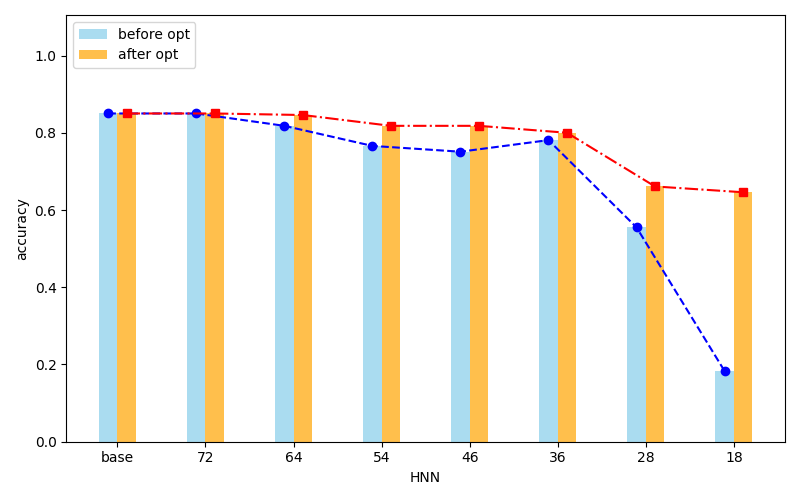
\includegraphics[width=0.8\textwidth]{优化对比.png}
  \bicaption[优化前后模型性能对比]{优化前后模型性能对比}{Comparison of Model Performance Before and After Optimization}
  \label{fig:优化前后模型准确率对比}
\end{figure}
图\ref{fig:优化前后模型准确率对比}实验结果表明,基于大规模训练数据构建的投影矩阵$V$可显著提升本征正交分解(POD)的模型压缩效果,其优化效果与降维程度呈正相关。当隐藏层维度压缩至36以下时(对应压缩比大于65\%),优化后模型的分类准确率较未优化基线平均提升1.9\%,验证了高维状态空间中关键维度的统计特性对压缩性能的关键影响。进一步分析显示,单一训练样本构建的投影矩阵因覆盖状态空间有限,易受局部动态特征干扰,导致压缩模型泛化能力下降,而基于多批次数据联合优化的投影矩阵,能够有效提取共性特征,特别在当维度降低至36以下,数据已丢失关键信息维度时,能够显著提高压缩后的模型性能。这一现象表明,投影矩阵的泛化性能本质上取决于训练数据分布的覆盖范围,当样本量不足时,POD易陷入局部最优解,而大规模数据驱动的策略可缓解非线性特征丢失的问题。

为证明POD算法的优越性,对比了现有对RNN类网络的压缩方式,与SVD\cite{xueRestructuringDeepNeural}方法进行对比,实验结果如表\ref{tab:method-comparison}所示。
\begin{table}[htb]
  \centering
  \begin{minipage}[t]{0.8\linewidth}
    \bicaption[方法对比结果]{方法对比结果}[Comparison results]{Comparison Results}
    \label{tab:method-comparison}
    \begin{tabularx}{\linewidth}{lXXX}
      \toprule[1.5pt]
      {\heiti 模型} & {\heiti 准确率(SVD)} & {\heiti 准确率(POD)} & {\heiti 压缩比(POD)} \\\midrule[1pt]
      基线 & 85.0\% & 85.0\% & - \\
      HNN=72 & 85.0\% & 85.0\% & - \\
      HNN=64 & 62.9\% & 84.6\% & 93.5\% \\
      HNN=54 & 61.8\% & 81.8\% & 73.7\% \\
      HNN=46 & 33.7\% & 81.8\% & 52.3\% \\
      HNN=36 & 35.5\% & 80.0\% & 34.4\% \\
      \bottomrule[1.5pt]
    \end{tabularx}
  \end{minipage}
\end{table}

首先在模型的准确率上,POD方法和SVD方法在没有后续微调的静态对比实验中,性能明显优于SVD方法;其次在压缩效率上,SVD方法通过将系数矩阵低秩分解为两个矩阵并利用参数共享来减少参数,这种方法在压缩至同样的隐藏层节点上,压缩效率远远不及POD方法,并且只有在隐藏层节点数小于原始节点数量的一半时才有明显压缩效果,并且SVD方法通过两个低秩矩阵近相乘似一个系数矩阵时,会额外增加模型的计算量,而POD方法在保证压缩效率的同时也显著降低了模型推理时的计算量。因此,POD方法在模型精度、压缩效率和计算量三个层面均优于SVD方法。由于POD方法只在模型内部降低维度,输出维度与原始模型不变,所以当模型应用于文本嵌入等任务时,可以在不降低文本嵌入维度的前提下进行模型的压缩和加速。对于多模型合作任务下,能够保持输入输出向量为度不变,在压缩后不需要改变前后模型的输入输出维度,节省了计算资源,提高了计算效率。
\section{本章小结}
本文提出了一种新的模型压缩方法,基于模型降阶方法——本征正交分解法来压缩循环神经网络。该方法可使原始模型具有最优的隐藏节点数,用较小的模型尺寸实现较高的准确率。实验中原始模型很小,总参数只有60k,因此可以将其视为紧凑模型。紧凑模型比参数规模较大的稀疏模型更难在不损失精度的情况下进行压缩。如果紧凑模型的精度损失可以控制在5\%以内,稀疏模型也可以用同样的方式在精度损失更小的情况下压缩模型参数。提出的方法可以应用于长短期记忆网络等具备时间序列特征的神经网络的压缩任务。这种新方法可以将模型大小减少到三分之一,将计算量减少到四分之一,并在精度上将损失控制在5\%。这同时也是一种不经过微调的直接调整网络结构的方法,因此它也可以与权重量化等压缩方法相结合,构建一个紧凑高效的模型。通过动力学系统的模型降阶方法来分析神经网络模型并对其压缩,也增加了对神经网络模型的解读视角和可解释性。

本章内容已发表会议论文并EI检索。

% !Mode:: "TeX:UTF-8"
\chapter{基于大模型的表格数据检索增强与推理优化}
\label{cha:第四章}
本章节主要以大模型在表格数据推理以及实际应用场景进行了深入的研究,提出了一种多级表格检索增强方法和大模型的表格推理框架,解决了检索增强推理任务中对表格文件的召回率低和大模型对表格数据推理能力差的问题。并将其应用于水利水库调度业务场景,构建水利水库调度场景下的基于大模型的智能反馈交互系统。
\section{问题描述}
结构化表格数据作为信息组织与存储的关键形式,在企业数据库、科研记录、金融报表等诸多领域有着广泛且深入的应用。在当今数字化转型加速的时代背景下,数据驱动的决策制定、业务流程优化以及知识发现等活动,愈发依赖于对结构化表格数据的高效利用与深度挖掘。

大型语言模型(LLMs)凭借其强大的语言理解和生成能力,已经在自然语言处理领域取得了显著成就。然而,传统LLMs在处理结构化表格数据时存在明显局限性,主要表现为对表格数据的结构化特征理解不足,难以有效执行复杂的数值计算、数据关联以及逻辑推理等任务。这在很大程度上限制了LLMs在众多实际应用场景中的进一步拓展与深化。这种能力的提升对于拓展大模型在真实场景中的实用性具有至关重要的意义。在数据分析方面,模型可以更高效地从海量表格数据中提取有价值信息,生成具有深度理解的分析报告;在决策支持场景中,模型则能够基于表格数据进行复杂的情景模拟与预测分析,为决策者提供科学、可靠的依据,助力其做出更明智的决策。
\section{表格数据推理框架的搭建}
表格数据具有复杂的行列关系、数值精度高、规模庞大等特点,传统LLM易受上下文长度限制、高token消耗和数字语义解析能力不足的影响。研究大模型表格推理方法(如程序生成、检索增强)能有效解决这些问题,提升模型对结构化信息的处理效率和能力。目前主流的大模型表格数据推理方法是借助代理Agent思想,将问题中的数据分析任务和语义理解等任务剥离,将任务拆分为各个子任务,代码生成任务为最关键的一步,根据任务需要生成可执行的代码,再通过外部接口对表格执行如SQL、python等机器语言来简化表格内容,降低任务难度,进而提升大模型对表格推理能力。

该研究主要面临两个困难和挑战,首先是大模型对数字文本的理解推理能力不足,如图\ref{fig:4-1}所示,大模型无法理解多个数据之间的数量大小关系,无法进行准确的数学计算,以至于对关键数字信息的提取和处理出现错误;二是对于庞大的表格数据,直接将结构化表格文本线性化的方法会产生过长的上下文,从而超出模型的最大上下文长度,从而截断表格,导致信息缺失降低回答质量。并且大模型处理过于复杂和冗长的上下文信息时,会因为无法识别关键信息而出现幻觉问题。综上所述,要提高大模型对表格数据的处理能力需要完成两个工作,一是将表格中复杂的数据关系和计算任务通过外部工具实现,二是剔除表格中与问题无关的冗余数据,只留下关键数据降低推理负担,从而提高大模型的推理能力。
\begin{figure}[!htbp]
    \centering
    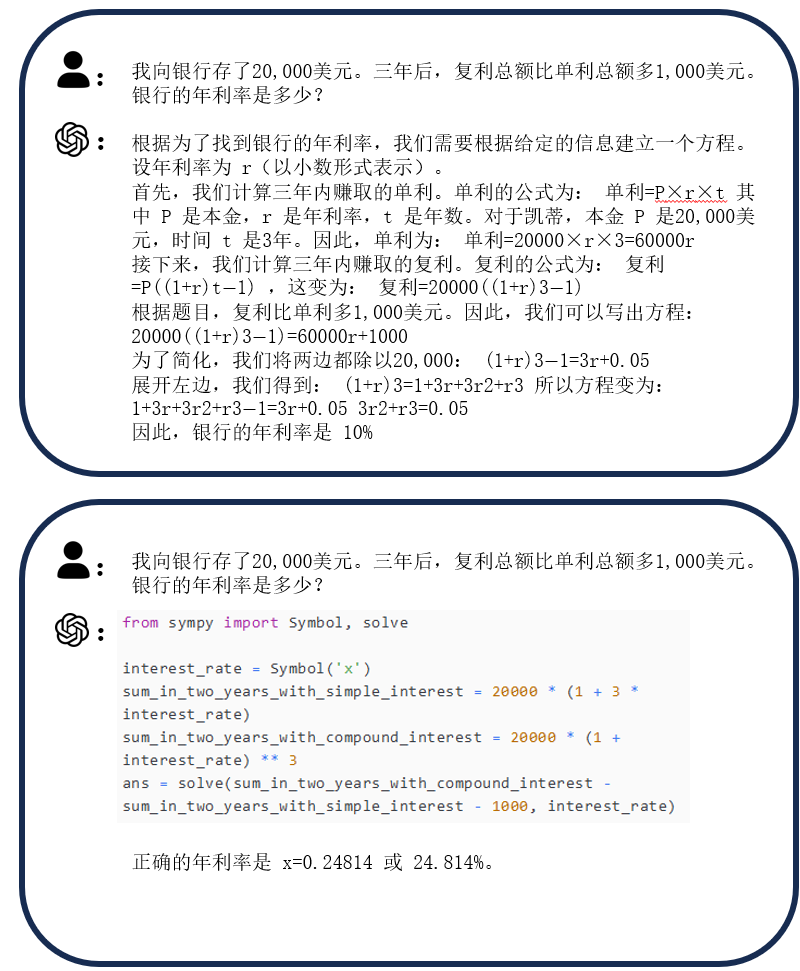
\includegraphics[width=0.7\textwidth]{大模型对数学问题的处理结果.png}
    \bicaption{大模型对数学问题的处理结果}{Results of Mathematical Problem Processing by LLM}
    \label{fig:4-1}
\end{figure}
同时,面对实际数据分析任务,表格数据输入模态多种多样包括excel表格、纯文本形式表格、数据库database表格和PDF表格等。针对多模态的表格文件主要存在两种处理方式,一种是将所有模态表格均以图片的形式输入大模型\cite{zhengMultimodalTableUnderstanding2024},利用了LLaVA、Vit\cite{bangMultitaskMultilingualMultimodal2023,chenCLIP2SceneLabelefficient3D2023,liuVisualInstructionTuning2023,radfordLearningTransferableVisual2021,dosovitskiyImageWorth16x162020}等视觉编码模型将表格编码输入大模型,是一种端到端的方法,该方法即使在部分任务的表现上达到了最优,但是该方法缺乏可解释性、消耗计算资源过于庞大且依然不能解决大模型对数字信息的计算和推理能力;第二种方法是利用Agent代理的思想,利用外部接口来代替大模型处理数学问题并简化表格文件,提取关键信息。利用代理思想的方法拓展了大模型在解决问题时的功能多样性,将多种大模型不熟悉的如数字运算、数字推理等任务统一转化成代码生成任务,即大模型最擅长的任务。代理方法相对视觉编码的方法节约了大量训练算力,并且提高了大模型在任务中的可观测性和可解释性,是实际应用中的主流方法。
\subsection{多级表格数据检索构建}
该方法主要包括对复杂表格数据的预处理、大模型的多轮推理以及外部SQL接口的使用。目前的主流表格推理框架默认所推理表格与问题的相关性,直接将具备回答问题所需信息的表格作为输入,测试框架的推理能力。但是在实际的推理任务中,需要通过文本向量相似性等方法对目标表格进行召回,为了提高召回精度同时保证大模型的推理的后续推理能够顺利进行,下面本章节提出一种多级表格数据目录检索方法。

由于表格数据的数据结构特点,使用RAG系统中传统的文本预处理切块方式会导致表格的召回率不高和召回表格不完整。对于传统文件处理方式,将表格数据以文本方式使用切块方法将表格以多个文本块的形式向量化存储在向量数据库中。由于表格文件的大部分信息均为数字,如果表格在中间截断,表格的中间部分以响亮的形式存在,没有表头和表名,数据会丧失意义和信息。同样不同表格的中间数据部分会有相似的情况,若直接使用文本相似度检索非常容易将不同表格的数据信息混淆,导致信息失真,进而影响回答质量。表格数据之间相互区别的主要信息主要为表名和表头,这两个特征赋予数字实际意义,所以希望根据表头和表名信息构建数据向量库,同时也能够避免表格数据因长度过长被分割后,单独的数字信息丧失实际意义的问题。同时将过长的表格数据存储在向量数据库中也会在召回时浪费大量的相似度计算资源和延长响应时间。综上所述,本文设计了只将表名和表头向量化存储在向量数据库中,把表格的数据信息通过JSON和database的形式存储在本地,根据向量化检索后的metadata进行本地表格定位,并且根据不同表的特征进行优化的表格召回方法。该方法可以提高召回率和召回效率,并且可以保证将完整表格输入给大模型推理,同时为后续推理优化方法提供了格式化的表格文件。
\begin{figure}[!htbp]
    \centering
    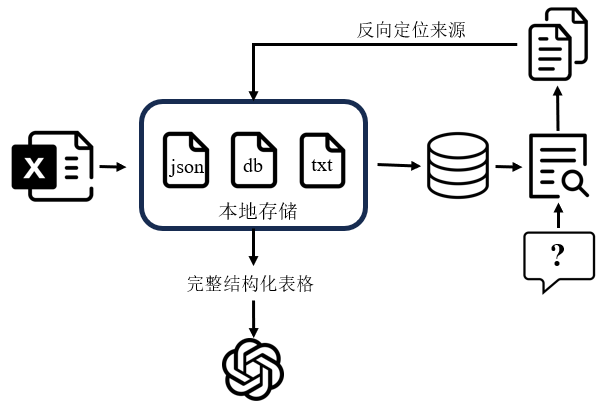
\includegraphics[width=0.66\textwidth]{表格检索框架示意图.png}
    \bicaption{表格检索框架示意图}{Schematic Diagram of Table Retrieval Method}
    \label{fig:4-2}
\end{figure}
将表格文件转化为JSON、database和txt文本形式存储,再将txt文件中的表名和表头文本嵌入向量化,此时在向量数据库中,每一条对应的表头信息都包含一个特征metadata,即这个向量数据是由哪个文件向量化而来。当输入的问题通过向量搜索模型匹配到目标表格时会直接定位到本地原始文件,根据需要提供JSON文件和database文件给后续框架进行推理等操作。在向量检索中使用双塔检索结构\cite{bahdanauNeuralMachineTranslation2016,sutskeverSequenceSequenceLearning2014,radfordImprovingLanguageUnderstanding2018,fanHierarchicalNeuralStory2018,holtzmanCuriousCaseNeural2020}。在召回过程中,双塔检索结构通过分阶段优化效率与精度,通常分为粗召回(Candidate Generation)和精排序(Re-ranking)两个层级:粗召回阶段采用双塔神经网络架构,其中查询侧(Query Tower)和候选侧(Item Tower)分别通过独立编码器如Transformer,将问题文本编码为词向量,其中候选侧的编码过程为离线进行,在向量库构建时完成。再通过向量内积或余弦相似度计算初步匹配得分,并借助近似最近邻搜索(ANN)快速筛选Top-K候选集,实现计算效率与召回覆盖率的平衡;精排序阶段则引入复杂模型如第\ref{chap:第二章}章中介绍的BERT模型,对粗召回结果进行精细化相关性评估与排序,直接通过端到端的方式将问题和粗召回的候选向量输入,由模型输出相似度得分,从而在可控计算成本下提升整体召回质量。两阶段分工耦合,形成“高效粗筛-精准判别”的递进式检索范式,兼顾系统响应速度与语义匹配深度。由于向量库中的数据庞大,如果直接使用端到端方式筛选合适文本表格会耗费大量的计算资源和时间,所以会提前通过比较文本相似的的方式以离线的方式将数据嵌入,但只依赖这种方法无法保证搜索到准确性,所以使用了先召回后精排的搜索方式。
\subsection{循环推理框架构建}
如上文提到,如果直接将上小节引入的检索方法检索到的表格输入给大模型会存在表格过长超出模型最大上下文长度和大模型对表格数据推理能力差的问题。可以通过引入Agent代理思想,通过SQL执行来处理表格,通过将数据精简减少表格长度和推理难度的方式提高回答质量,同时也使用SQL的计算能力来弥补大模型对数字关系推理的不足。

Agent代理的核心思想之一是将复杂任务分解为多个简单任务,从而降低每一次大模型调用时面对任务的难度,进而提升回答质量。是由多个大模型分工合作共同完成一次推理任务。综上所述,提出一种大模型循环表格推理框架,利用大模型强大的代码生成能力和自纠错能力生成准确有意义的SQL代码,再由外部接口执行代码并循环以上操作,得到最后精简的数据供大模型推理生成最终答案。

单次调用大模型生成SQL结果需要统一格式并且尽量降低模型的输出丰富度,可以通过调整模型输入参数和设计特殊提示词模板来实现,模型可以通过temperature参数控制输出的丰富程度,temperature越高,生成的文本更多样,反之,生成的文本更确定,因此对于生成SQL的大模型temperature设置为0.8,因为既需要固定同一个表格同一个需求输出SQL的一致性,也需要适当提高针对同一个表格不同需求的多样性。而针对固定大模型的输出格式上,框架希望可以直接将输出的文本作为下一阶段推理的输入,所以需要输出为可直接运行的SQL代码。上述需求通过提示词来解决。

提示词作为大模型调用的关键一环,可以不经过训练只使用文字输入的形式让大模型了解任务的需求,具体原理介绍已经在第\ref{chap:第二章}章写明。在SQL生成的提示词中,需要满足以下要点:

首先明确提出任务需求,该大模型的推理任务是什么。其次令模型理解输入的表格具体结构。因为检索到的目标表格也是以提示词的形式作为输入给大模型,这涉及到上面提到的表格篇幅过长问题,既需要令大模型明白表格的全貌,又需要减少表格长度。这里同样借助SQL的能力,利用SQL中表格初始化代码代替整张表格来使大模型理解表格结构,同时将大模型的知识注意力引入SQL中,再截取表头和少量表格信息组成提示词。在生成可直接运行的SQL代码的过程中,若采用冗长的文本描述方法,会存在以下问题:一方面受限于文字表达能力的局限性,难以精准且简洁地描述SQL代码的生成逻辑与结构;另一方面,模型在理解与转化这些文本描述时,存在一定概率出现语义对齐不准确的问题,导致生成的SQL代码无法准确实现预期功能。为解决这一问题使用Few-shot learning少样本学习方法,通过少数训练样本直接以提示词的形式来规范输出格式。设计满足以上需求的提示词如图\ref{fig:4-3}所示。
\begin{figure}[!htbp]
    \centering
    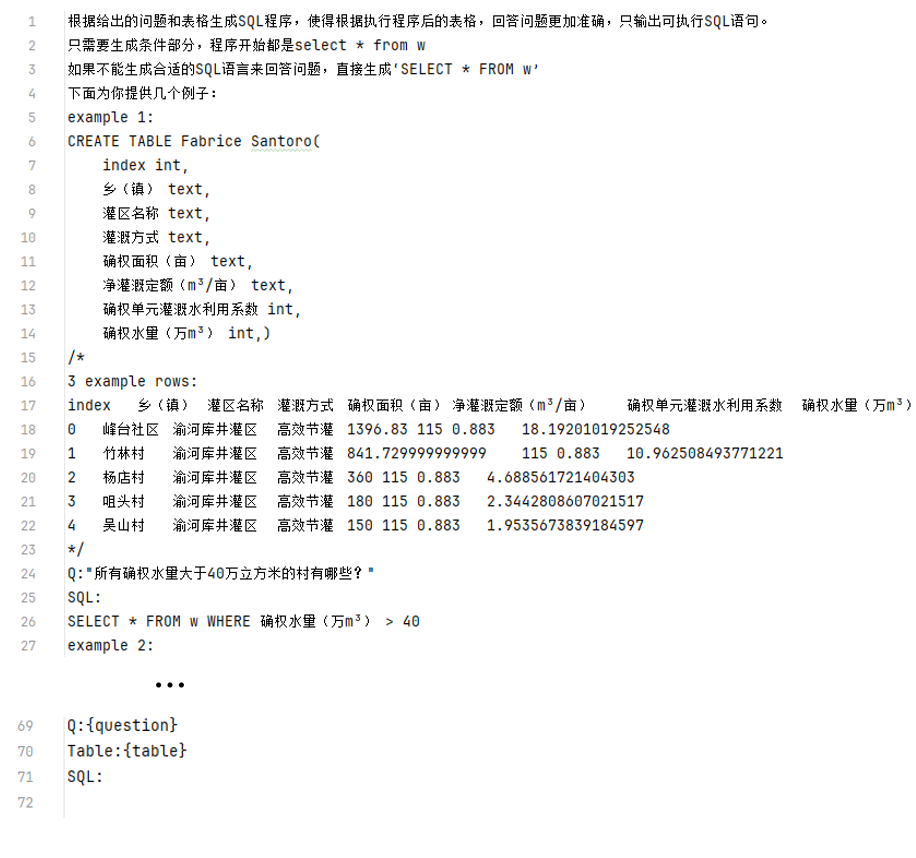
\includegraphics[width=0.95\textwidth]{SQL生成任务提示词.png}
    \bicaption{SQL生成任务提示词}{SQL Generation Task Prompt Words}
    \label{fig:4-3}
\end{figure}

提示词模板最后通过字典的格式将问题和文本化表格嵌入,由于少量输入输出例子,大模型会优先模仿并跟随前面的输出,就能保证输出SQL语句的一致性。
\begin{figure}[!htbp]
    \centering
    \includegraphics[width=0.79\textwidth]{无few-shot.png}
    \bicaption{无少样本学习的SQL生成}{ SQL generation without Few-shot learning}
    \label{fig:4-4}
\end{figure}
特别注意的是,嵌入提示词模板的表格数据都将是以图\ref{fig:4-3}中一样文本的形式,包括最后生成回答的推理过程,database的文件形式只用于在框架内部利用SQL生成简化后的表格。然而还是有概率会出现输出SQL命令执行出错的问题如下图\ref{fig:4-5}所示。这里需要利用大模型的代码理解能力与自纠错能力,设计一种大模型的多循环自反馈框架。
\begin{figure}[!htbp]
    \centering
    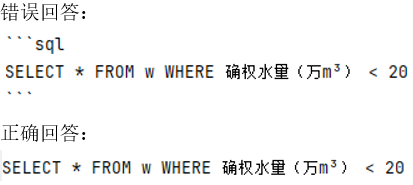
\includegraphics[width=0.5\textwidth]{SQL生成对比.png}
    \bicaption{SQL生成对比}{Comparison of SQL Generation}
    \label{fig:4-5}
\end{figure}

该框架中设计的为三次循环反馈的自适应错误修正框架,其核心机制在于构建动态上下文感知的自纠正系统。将每次执行输出报错后的系统报错与前文组成上下文,生成包含完整错误的增强型上下文再输入模型。经过实际测试,将往次输入的报错和纠正共同组成上下文输入给模型非常关键,这样有助于令大模型意识到自身的错误方向和改进方向,若每次的报错信息单独输入给大模型会导致其原地踏步,孤立地处理离散错误事件。
\begin{figure}[!htb]
    \centering
    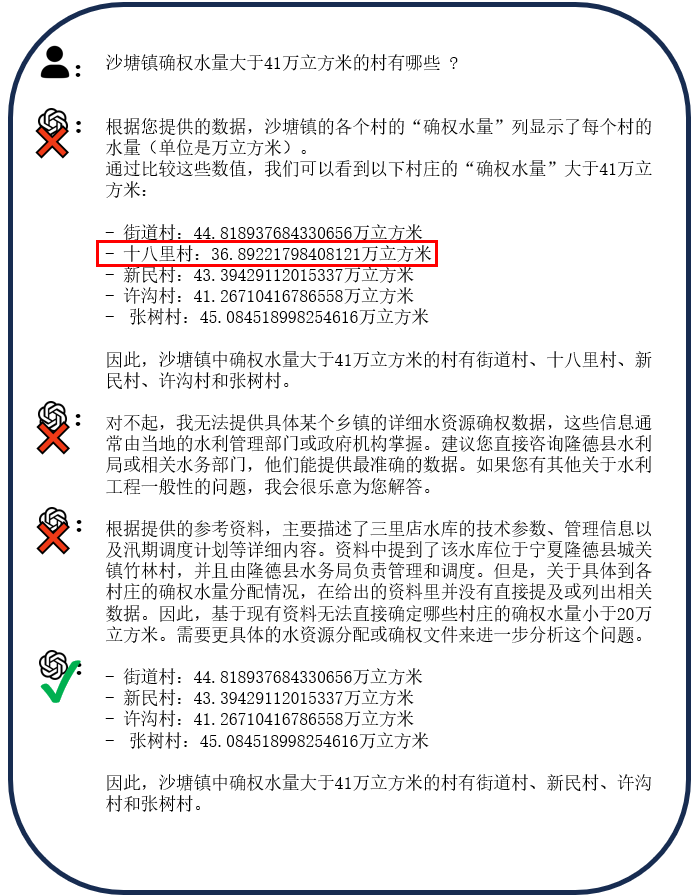
\includegraphics[width=0.8\textwidth]{回答对比.png}
    \bicaption{优化前后回答对比}{ Comparison of Answers Before and After Optimization}
    \label{fig:4-7}
\end{figure}
当系统经历完整的三次迭代仍未能达成有效修正时,系统自动切换至为无优化的基础查询模式,直接执行select * from w全表扫描指令,将全部表格输出给下一步推理,来确保系统输出的完整性。这种双重模式切换机制在保证框架鲁棒性的同时,有效规避了因循环修正导致的潜在计算资源浪费问题。整体过程如图\ref{fig:4-6}所示。
\begin{figure}[htbp]
    \centering
    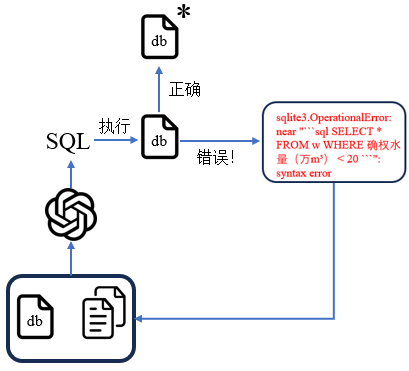
\includegraphics[width=0.63\textwidth]{循环反馈示意图.png}
    \bicaption{循环反馈示意图}{Schematic Diagram of Feedback Loop}
    \label{fig:4-6}
\end{figure}

\section{反馈信息优化对比}
针对表格的信息查询任务测试,如图\ref{fig:4-7}所示。测试涉及对目标表格“隆德县农业灌溉用水确权汇总表”的召回和单特征数量关系的筛选。第一个回答为返回目标表格但无SQL优化回答,在回答中出现了错误答案,误将确权水量为36万立方米的十八里村输出;第二个回答由于在召回过程中,所有的向量相似度过低没有达到阈值,无表格返回;第三个回答为返回错误表格“三里店水库汛期调度运用计划表”导致,最后的回答经过两次优化得到的正确召回目标表格并通过SQL优化后得到正确数据并返回后的结果。

针对表格检索任务,由水利局专家设计构造了针对隆德水库信息查询的问题集并对本章提出的多级表格检索方法和不进行特殊处理直接使用FAISS内部向量化嵌入方法进行对比测试。在测试中为了避免表格超出上下文长度导的致表格截断问题,只统计在大模型最大上下文长度内的表格与对应问题,测试结果如表\ref{tab:table-retrival-results}所示。可以看出,本章提出的多级表格检索方法在召回率上有明显提升,提高了表格数据的召回率。
\begin{table}[htbp]
    \centering
    \bicaption{表格检索实验结果}{Table Retrieval Experiment Results}
    \label{tab:table-retrival-results}
    \begin{tabularx}{\linewidth}{XXX}
        \toprule[1.5pt]
        \textbf{方法} & \textbf{原始方法} & \textbf{多级表格检索方法} \\
        \midrule[1pt]
        返回情况 & 91/110 & 105/110 \\
        \bottomrule[1.5pt]
    \end{tabularx}
\end{table}

\section{本章小结}
本章节主要探讨了基于大模型的表格数据推理框架的设计,旨在提升大模型对结构化表格数据的理解与推理能力。通过深入分析表格数据的特点及大模型在处理表格数据时面临的挑战,提出了一种结合多级表格数据检索与循环推理的框架。

首先,针对表格数据的复杂性和大模型的局限性,设计了一种多级表格数据检索方法。该方法通过将表格的表名和表头信息向量化存储,避免了表格数据因长度过长而被分割的问题,提高了表格数据的召回率和召回效率。
其次,提出了一种大模型循环推理框架,通过引入Agent代理思想,将复杂任务分解为多个简单任务,降低了每次大模型调用时的推理难度。该框架利用大模型的代码生成能力,生成可执行的SQL代码,通过外部接口执行代码来简化表格数据,弥补了大模型在数字推理能力上的不足。此外,设计了一种多循环自反馈机制,通过动态上下文感知的自纠正系统,提高了推理的准确性和鲁棒性。

通过上述方法,本章成功构建了一个高效的表格数据推理框架,显著提升了大模型在处理结构化表格数据时的性能。这一框架不仅优化了表格数据的检索和推理过程,还为实际应用中的智能反馈交互系统提供了强有力的技术支持。

本章所述内容已应用于学校合作企业的相关技术研发,并已提交专利申请。

% !Mode:: "TeX:UTF-8"
\chapter{基于大模型的智能反馈交互系统设计}
\label{cha:第五章}

随着大模型技术的逐渐成熟,各个行业开始利用大模型的优秀生成能力完成简单工作。本章节主要介绍第\ref{cha:第四章}章的表格推理框架在学校与隆德县水利局合作项目中的应用,该项目主要设计研发面向水利调度领域的基于本地知识库的大模型智能反馈交互系统。该反馈系统的目的在于利用大模型推理和文本向量检索技术帮助水利行业从业者迅速掌握专业知识,面对多变的水利问题提供专家建议,节约学习和用人成本,减少因人为因素导致的工作失误,提高工作效率。该反馈系统主要通过检索增强推理技术(Retrieval-augmented Generation, RAG)对复杂庞大的水库信息和水利调度经验进行分析,生成从业人员需要的专业意见。本智能反馈交互系统主要包括两个部分,本地知识库的构建和基于知识库的智能问答功能。
\section{系统关键技术框架及应用}

智能反馈交互系统的工程实现主要包含以下功能模块:1 、向量数据库的构建及向量搜索2、基于大模型的推理框架。下面对工具开发中涉及的核心框架进行简单介绍。

LangChain作为当前最先进的智能化应用开发框架,其核心价值在于构建基于大语言模型(Large Language Model, LLM)的端到端应用系统。该框架采用模块化架构设计,提供标准化接口实现模型与外部组件的协同工作。从技术架构层面分析,LangChain包含模型交互(Models)、数据检索(Indexes)、链式流程(Chains)、记忆模块(Memory)和智能体(Agents)五个核心子系统,支持通过组合式编程构建复杂的人工智能应用。其独特的链式调用机制(Chain Invocation Mechanism)允许将多个LLM操作、工具调用及数据处理流程进行有序编排,在对话系统、知识问答、文档分析等场景展现出显著优势。

本研究选择LangChain框架主要基于其三大核心优势:首先,该框架通过标准化接口设计有效解决了大语言模型与外部系统的集成难题,提供与OpenAI、Hugging Face等主流模型平台的即插即用式对接方案;其次,其模块化设计支持灵活的功能扩展,特别是在处理长文本、多轮对话等复杂场景时,可通过记忆模块实现上下文状态的持久化存储;最后,LangChain内置的检索增强生成(Retrieval-Augmented Generation, RAG)技术架构,为构建基于私有知识库的智能问答系统提供了完整的技术实现路径。

FAISS\cite{johnsonBillionscaleSimilaritySearch2019}(Facebook AI Similarity Search)是由Facebook AI Research团队开发的一个开源库,用于高效的相似性搜索和密集向量聚类。它能够在大规模数据集上进行快速的相似度搜索,即使这些数据集不适合在内存中加载。FAISS提供了多种索引类型,每种索引都有不同的适用场景和性能特点。它支持多种相似度度量方法,包括L2距离、内积相似度等,能够满足不同场景下的需求。FAISS还支持GPU加速,可以显著提高查询速度,特别是在处理非常大规模的数据时。它广泛应用于推荐系统、搜索引擎、自然语言处理等领域。

LangChain与FAISS的技术组合在本研究中展现出显著的协同优势。从系统架构视角,LangChain的RetrievalQA链(Retrieval-Enhanced Q\&A Chain)通过整合FAISS的语义检索能力,构建起“检索-排序-生成”的三阶段处理流程,使生成式模型的准确率提升。在工程实现层面,两者的深度集成体现为:FAISS负责将PDF文献、实验数据等非结构化文档转换为向量并建立多模态索引,而LangChain则通过自适应的查询路由(Query Routing)机制,动态选择最优检索策略。该技术方案的选择同时考虑了学术研究价值与工程实践需求:在理论层面,二者的结合验证了检索增强生成模型在垂直领域知识库中的应用可行性;在实际设计方面,FAISS和langchain具备优秀的系统可扩展性,能够简单适配系统中其他功能模块,节约了大量的开发成本。

为实现本文中介绍的表格优化推理框架方法,需要借助外部数据库功能。具体使用的数据库接口为SQLite。其是一款轻量级、无服务器、自给自足的关系型数据库管理系统,其设计理念强调嵌入式应用的简洁性与高效性。SQLite通过将整个数据库系统以单一磁盘文件形式实现,显著降低了部署复杂度与资源消耗,相较于传统数据库,SQLite在内存占用(仅需数百KB)与计算资源需求方面具有显著优势。以上优势支撑其作为推理过程中充当执行SQL的辅助功能,能最大限度地提高推理速度。

\begin{table}[htb]
    \centering
    \begin{minipage}[t]{0.75\linewidth}
      \bicaption[具体使用模块]{具体使用模块}[Specific Usage Modules]{Specific Usage Modules}
      \label{tab:modules}
      \begin{tabularx}{\linewidth}{XX}
        \toprule[1.5pt]
        {\heiti 模块} & {\heiti 名称} \\ 
        \midrule[1pt]
        向量数据库    & FAISS \\
        粗召回模型    & qwen-text-embedding-v2 \\
        精排序模型    & bce-reranker-base\_v1 \\
        Database     & SQLite \\
        LLM          & qwen-max \\
        前端界面     & streamlit、vue \\
        \bottomrule[1.5pt]
      \end{tabularx}
    \end{minipage}
  \end{table}
在框架中使用的大模型组件为阿里云的通义千问系列大模型中的qwen-max\cite{baiQwenTechnicalReport2023}, 在通义千问系列中性能表现最佳,中英文code能力、逻辑能力、多语言能力显著提升,回复风格面向人类偏好进行大幅调整,模型回复详实程度和格式清晰度明显改善,创作类专项、JSON格式遵循专项、角色扮演专项能力定向提升。文本嵌入的粗排序模型同样使用通义千问系列的text-embedding\_v2模型,将本地知识库嵌入为向量数据库、对系统输入进行向量化和对检索召回的文本向量进行解码,输出可阅读的文本信息。而对于精排序模型使用网易bce-reranker-base\_v1\cite{BCEmbeddingREADME_zhmdMaster}模型,直接计算问题输入与粗排序模型返回的部分文本向量之间的相似度,提高检索召回率。

\section{RAG智能反馈交互功能设计}
本章详细介绍了智能反馈交互系统中的对知识库的问答反馈功能。该功能主要基于检索增强生成(RAG)技术,将隆德县水库信息、水利调度专家经验、专业文档以及规章制度等封闭领域知识,以搜索提示词的形式输入模型进行推理。尽管通用大模型在处理广泛领域的知识和文本理解方面表现出色,但在应对知识密集型和封闭领域的问题时,往往难以发挥其应有的功能,如图\ref{fig:无检索}所示。
\begin{figure}[!htb]
    \centering
    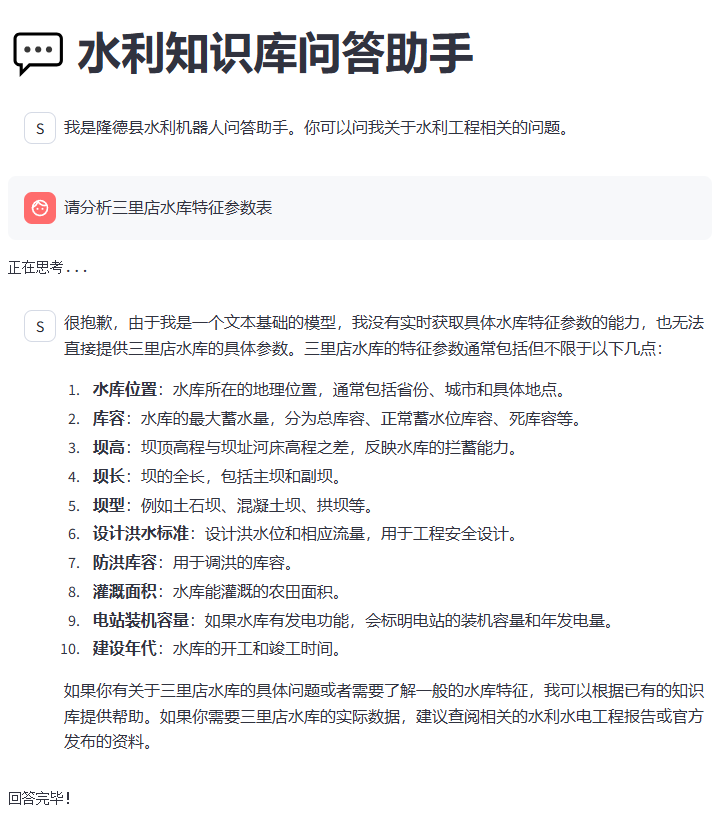
\includegraphics[width=0.8\textwidth]{无检索回答.png}
    \bicaption[无专业知识大模型回答]{无专业知识大模型回答}[Answer to the Large Model Without Professional Knowledge]{Answer to the Large Model Without Professional Knowledge}
    \label{fig:无检索}
\end{figure}
当面对特定的水利问题时,通用大模型通常无法提供准确的回答,这主要是由于其训练方式的局限性所致。此外,由于行业内封闭知识不对外公开,大模型无法通过常规训练途径获取这些知识。鉴于通过训练大模型来获得这些知识的计算成本和训练难度极高,因此选择将这些知识以提示词的形式输入大模型,以实现大模型对封闭领域知识的有效理解和应用。整体功能设计如图\ref{fig:rag整体结构图}所示。
\begin{figure}[h]
    \centering
    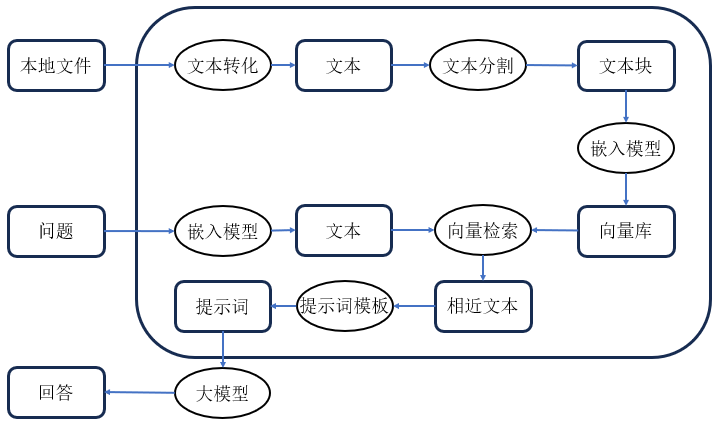
\includegraphics[width=0.75\textwidth]{rag整体结构图.png}
    \bicaption[RAG整体设计框架]{RAG整体设计框架}[Overall Design Framework of RAG]{Overall Design Framework of RAG}
    \label{fig:rag整体结构图}
\end{figure}
\subsection{向量数据库的构建}
在对水利局所辖的本地知识文件进行数据处理与分析过程中,发现其呈现出显著的格式异构性特征。具体而言,这些文件涵盖了多种不同类型的数据格式,包括Word文档、PDF文件、图像数据以及Excel表格等多元模态数据形式。针对其中的非结构化表格类文档,本研究采用了基于LangChain框架集成的OCR\cite{sarzynska-wawerDetectingFormalThought2021,tianDetectingTextNatural2016}(Optical Character Recognition,光学字符识别)文本提取接口,以实现对多模态数据的统一字符串转换,从而将图像中的文本信息以及其他非结构化数据转化为可处理的文本格式。

对于结构化表格文件的处理,则依据第四章所提出的结构化数据处理范式进行操作。其核心实现主要依赖于Python编程环境中的pandas数据分析库,通过该库强大的数据处理功能,能够有效地对结构化数据进行清洗、转换、分析以及可视化等操作,进而为后续的SQL生成与多级检索奠定坚实基础。
需特别指出的是,由于原始表格结构存在非规范化特征,许多文档在进行数据库转换时难以达到理想效果,如表\ref{tab:reservoir-scheduling}所示。即便数据以表格形式保存记录,但其内部缺乏多组信息之间的关联关系,本质上仅是利用部分表格结构来替代传统的文字叙述。

\begin{table}[htbp]
    \centering
    \bicaption[某水库部分调度计划表 ]{某水库部分调度计划表 }[Partial scheduling plan for a certain reservoir]{Partial Scheduling Plan for a Certain Reservoir}
    \label{tab:reservoir-scheduling}
    \begin{tabular}{|l|l|l|l|}
      \hline
      \multirow{6}{*}{泄水建筑物} & \multirow{3}{*}{开敞式溢洪道} & 型式 & 开敞式溢洪道 \\
      \cline{3-4}
      & & 进口高程(m) & 2061 \\
      \cline{3-4}
      & & 最大泄量(m³/s) & 114.9 \\
      \cline{2-4}
      & \multirow{2}{*}{最大泄量} & 断面尺寸(m) & 3.0×5.7 \\
      \cline{3-4}
      & & 最大泄量(m³/s) & 114.9 \\
      \hline
      \multirow{6}{*}{放水建筑物} & \multirow{3}{*}{水塔} & 型式 & 水塔 \\
      \cline{3-4}
      & & 闸门尺寸(m) & 1.0×1.0 \\
      \cline{3-4}
      & & 底坎高程(m) & 2051.7 \\
      \cline{2-4}
      & \multirow{3}{*}{涵管} & 断面尺寸(m) & 1.5×1.8 \\
      \cline{3-4}
      & & 最大泄量(m³/s) & 5.0 \\
      \cline{3-4}
      & & 最大泄量(m³/s) & 5.0 \\
      \hline
    \end{tabular}
  \end{table}
针对这种表格无法使用SQL来优化,但表格本身也不涉及到数学计算,表格长度较短,将这种表格称为结构化数据,通过JSON格式来增强文本结构化信息,如图\ref{fig:JSON}所示。形成由制表符文本到JSON再到database-SQL的三级存储形式。

\begin{figure}[!htb]
    \centering
    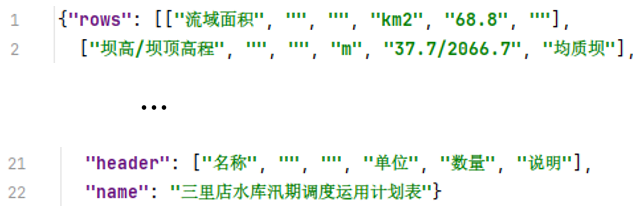
\includegraphics[width=0.8\textwidth]{json小.png}
    \bicaption[某水库部分调度计划表JSON格式]{某水库部分调度计划表JSON格式}[JSON form of Partial scheduling plan for a certain reservoir]{JSON Form of Partial Scheduling Plan for a Certain Reservoir}
    \label{fig:JSON} 
\end{figure}
\subsection{表格优化Agent设计}
在本研究构建的水利知识处理系统中,表格数据优化推理框架的流程图如图\ref{fig:SQL生成链}所示。该部分的核心功能在于:当本地知识召回的结果为表格文件时,利用第四章详细介绍的框架对召回的表格数据进行优化处理,并将优化后的表格数据输出给后续的流程,以供进一步的推理分析使用。这一过程对于确保数据的准确性和可用性至关重要,能够有效提升整个系统的推理分析效率和结果的可靠性。这部分是整个问答功能Langchain表达式的一部分。为了解问答助手的整体设计与Langchain的配合,需要对Langchain的基本功能组成单元LangChain表达式(LangChain Expressions,LCEL)进行介绍。LCEL是 LangChain 框架中一种基本类,能够通过直观串行或并行的方式将各个功能组合,能够由众多可以实现子功能的基本LCEL以下成为子链(sub-chain)串连或并联组成具备完整功能的链(chain)而每一个子链是由Langchain最小组成单位runnable类构成。在本功能的具体实施过程中,构建了一个以用户问题作为输入参数,并以经过简化处理的表格数据作为输出结果的子链结构。
\begin{figure}[!htb]
    \centering
    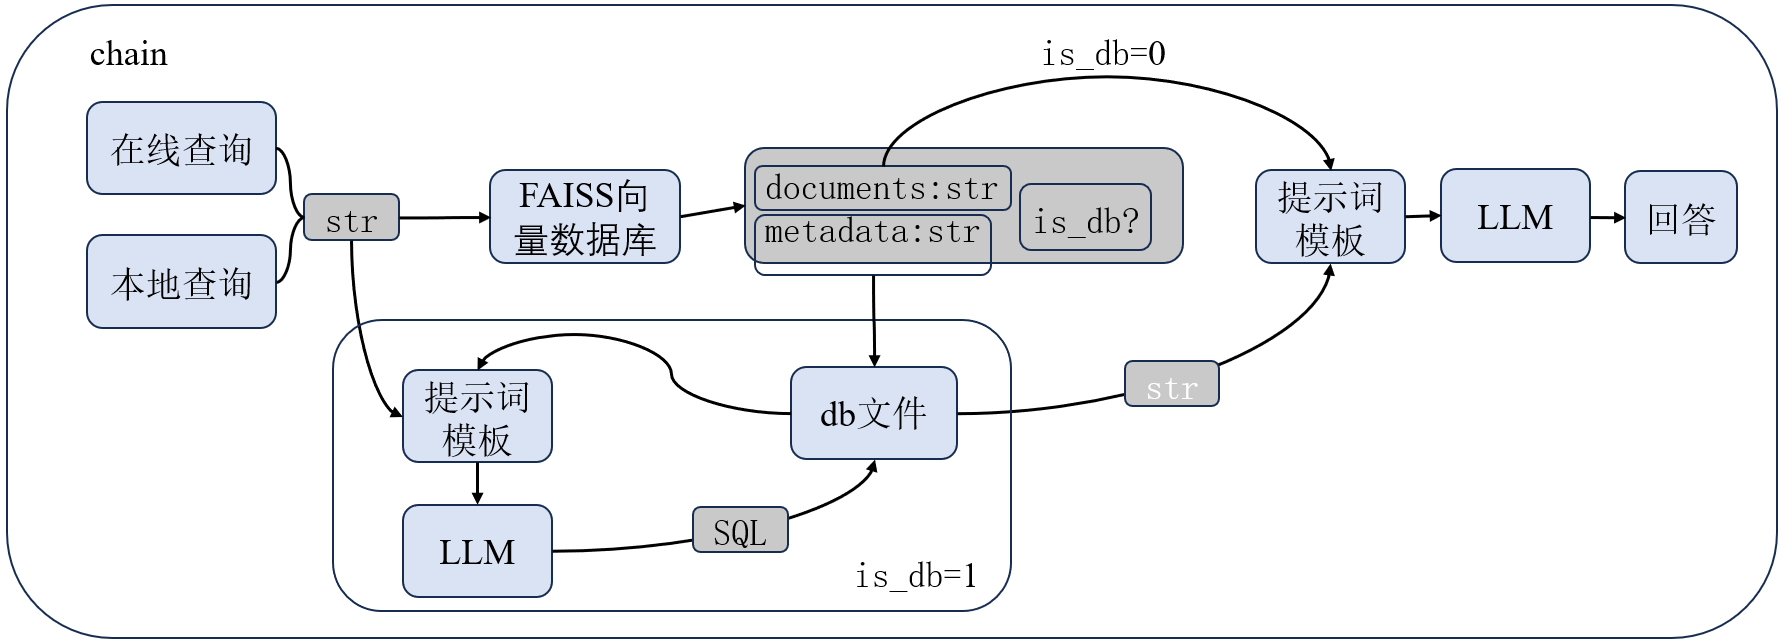
\includegraphics[width=0.9\textwidth]{SQL链生成示意图.png}
    \bicaption[SQL生成链示意图]{SQL生成链示意图}[SQL Generation Chain Diagram]{SQL Generation Chain Diagram}
    \label{fig:SQL生成链}
\end{figure}

在该子链的运行中,首先对 FAISS 向量数据库返回的 document 类别进行识别与处理。FAISS数据库进行两次检索,首先对向量库中的全部文本进行召回,此时使用的是文本相似度最邻近策略,将相似度最高的10个文本块(chunk)返回,在表格推理框架中则为10个表格文件,再由精排模型端到端地计算每个返回文本块与用户问题的相关性得分,取得分最高的文本块作为输出,当在本地环境中检测到第四章所介绍的三级存储结构时,系统会进一步判断是否可以采用 SQL 方法对表格进行优化。若判断结果为可行,则子链将生成相应的SQL语句并予以执行,随后将处理结果嵌入提示词模板,并输出给后续环节进行处理。反之,若判断结果为不可行,则子链将以结构化数据JSON的形式,将数据传递给后续环节,以确保数据的连续性和可用性。
\subsection{通用大模型推理功能设计}
在当前实现的功能中,问答反馈功能主要基于单轮问答机制,即每次交互仅针对一个具体问题提供答案。然而,为了满足更复杂的对话需求,问答反馈功能需要具备多轮问答功能。这要求系统能够记录上下文信息,以便在后续对话中引用历史内容。具体而言,历史对话以字典形式存储,其中包含三个关键字:“用户”(记录用户的提问)、“助手”(记录助手的回答)和“本地知识”(记录与对话相关的本地知识信息)。每轮对话的内容则以列表形式记录,以便于追踪对话的顺序和内容。

然而,在多轮对话和长文本检索的场景下,过长的上下文可能会对回答质量产生负面影响。这是因为新一轮对话未必与之前的每一轮对话及知识均存在关联性,过多的上下文信息可能会引入噪声,干扰模型的推理过程。为了解决这一问题,设计了一个子链结构,专门用于从历史上下文中检索与当前轮次对话相关的文本内容。该子链通过分析当前对话的主题和上下文,从历史记录中筛选出最相关的部分,从而确保模型在推理过程中仅参考有用的信息,提高回答的准确性和效率。这一机制的实现如图\ref{fig:多轮对话}所示,通过优化上下文管理,提升了多轮对话的整体性能。在上下文的文本检索过程中,为了提升系统的响应速度,仅采用单一的粗召回文本策略,并通过意图识别功能子链来判断在当前问答中是否需要在知识库中检索本地知识文档。

通过该子链,实际上将多轮问答任务转化为一种简化的形式,即通过提示词输入来替代传统的上下文传递方式,从而将多轮问答任务转化为单轮问答任务。这种设计既赋予了反馈系统多轮问答的能力,使其能够理解和处理多轮对话中的上下文信息,又保持了单轮问答任务在计算成本和推理难度方面的优势,降低了系统的复杂性和资源消耗。

\begin{figure}[!htb]
    \centering
    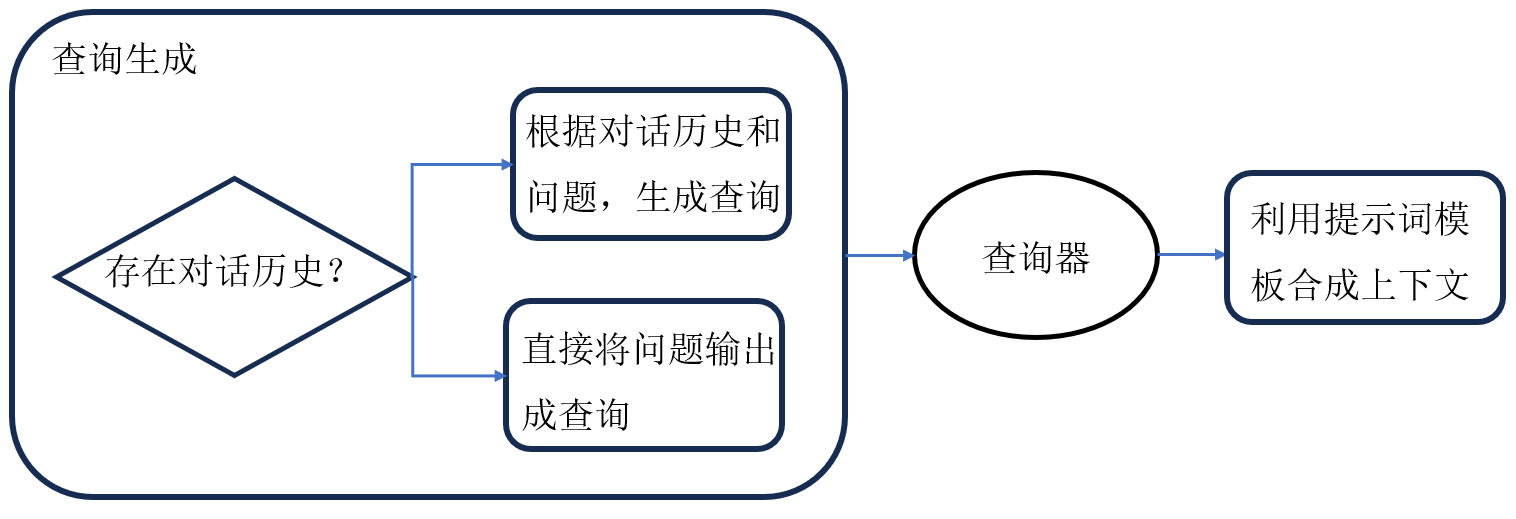
\includegraphics[width=0.88\textwidth]{对话历史生成流程图.png}
    \bicaption[对话历史生成流程图]{对话历史生成流程图}[Chat History Generation Flowchart]{Chat History Generation Flowchart}
    \label{fig:多轮对话}
\end{figure}
特别是对于直接将输出反馈给用户的环节,会将大模型的输出方式设置为流式输出(stream),即大模型的输出采用流式输出而非一次性输出所有答案,主要原因在于:一方面,流式输出能够逐步返回生成的中间结果,使用户能够更早地看到部分答案,减少等待时间,从而提升用户体验,增强交互的实时性和流畅性;另一方面,对于长时间的生成任务,一次性存储完整的输出会占用大量内存,而流式输出可以逐块返回结果,避免了一次性存储大量数据,从而降低内存占用。此外,流式输出能够适应实时应用需求,提供更自然的交互体验;同时,当输出内容较长时,一次性传输可能会导致请求超时,而流式输出可以分批次发送数据,降低超时风险,确保数据传输的稳定性。流式输出还可以模拟真实对话的输出节奏,让用户在AI生成回答时就能开始阅读,提前思考或及时打断对话,使交互过程更加流畅自然。

\section{知识库功能设计}

本小节希望通过建立业务规则库来支撑业务场景的规则适配,规范和约束水利业务管理行为,并同时以向量数据库的形式存储,为大模型反馈功能提供知识,如图\ref{fig:知识库流程图}。
\begin{figure}[htbp]
    \centering
    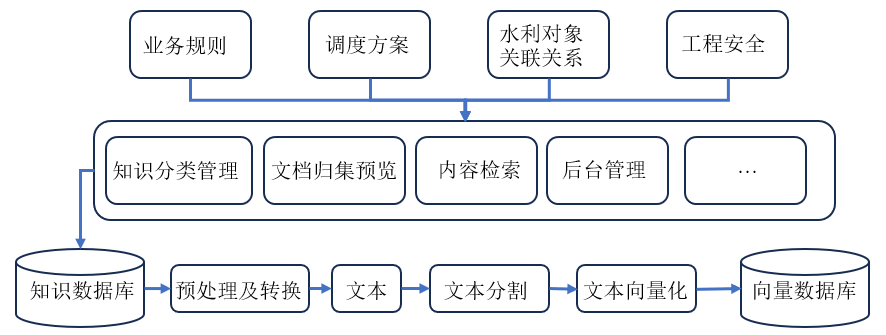
\includegraphics[width=0.9\textwidth]{知识库流程图.png}
    \bicaption[知识库流程图]{知识库流程图}[Knowledge Base Process Diagram]{Knowledge Base Process Diagram}
    \label{fig:知识库流程图}
\end{figure}
\begin{table}[htbp]
    \centering
    \renewcommand{\arraystretch}{1.2} % 调整行距
    \begin{minipage}[t]{0.8\linewidth}
        \bicaption[功能说明]{功能说明}[Function Description]{Function Description}
        \label{tab:功能说明}
        \begin{tabularx}{\linewidth}{l>{\centering\arraybackslash}X}
            \toprule[1.5pt]
            {\heiti 功能} & {\heiti 说明} \\
            \midrule[1pt]
      文档分类 & 对所有的文档进行分类,分类分级,在首页中可选择不同的分类查询对应的文档。 \\
      
      文档检索 & 提供强大的检索功能,支持全文检索、关键词检索、分类检索等多种检索方式,帮助用户快速找到所需文档。 \\
      
      文档下载 & 用户可以下载权限范围内的知识文档。 \\
      
      在线预览 & 对已经上传的文档在线预览,文件格式包括:.doc, .docx, .rtf, .odt, .dot, .fdf, .ppt, .pttx, .xls, .xltx, .csv, .chm, .txt, .pdf, .html。 \\
      
      文档管理 & 管理员可以对文档内容、类别、版本、属性、标签和权限进行修改和维护。 \\
      
      存储管理 & 提供安全、可靠的存储空间,用于存放知识库中的各类文件,如文本、图片、视频、音频等。 \\
      
      目录管理 & 根据知识库的内容和分类方式,设计合理的目录结构,包括一级目录、二级目录等,以便将知识内容进行归纳和整理。 \\
      
      标签管理 & 给知识添加标签,可以为其关联关键词或主题,便于用户快速筛选和查找相关内容。 \\
      \bottomrule[1.5pt]
    \end{tabularx}
\end{minipage}
\end{table}
调度方案库包括旱灾防御、水资源调度和管网爆漏应急等预案,并将调度预案进行分类保存;建立水利对象关联关系文档库,进行结构化分类和关联,便于水利知识的快速检索和定位;建立工程安全知识库,为工程安全管理提供知识服务,提高工程安全管理决策水平。
知识库文件管理功能主要包括以下几个方面:
1. 知识库分类与分级:对知识库进行分类和分级管理,便于用户根据需求快速
定位和查找相关知识文件。分类包括预报调度方案库、工程安全知识库、业务规则库
等,各分类下可分为不同级别。
2. 知识库文档管理:系统管理员可对文档进行维护上传、分类维护等操作,确
保知识库内容的完整性和准确性。
3. 知识库文件检索:提供模糊搜索功能,用户可通过关键词、文档标题、上传
日期等信息在知识库中快速检索所需知识文件。
4. 知识库文件在线预览与下载:支持多种文件格式的在线预览,如.doc、.ppt、.xls等。用户可在线预览文件,并根据需要进行下载。其他具体功能如表\ref{tab:功能说明}所示,图\ref{fig:知识库管理}为知识库的前端界面。
\begin{figure}[htbp]
    \centering
    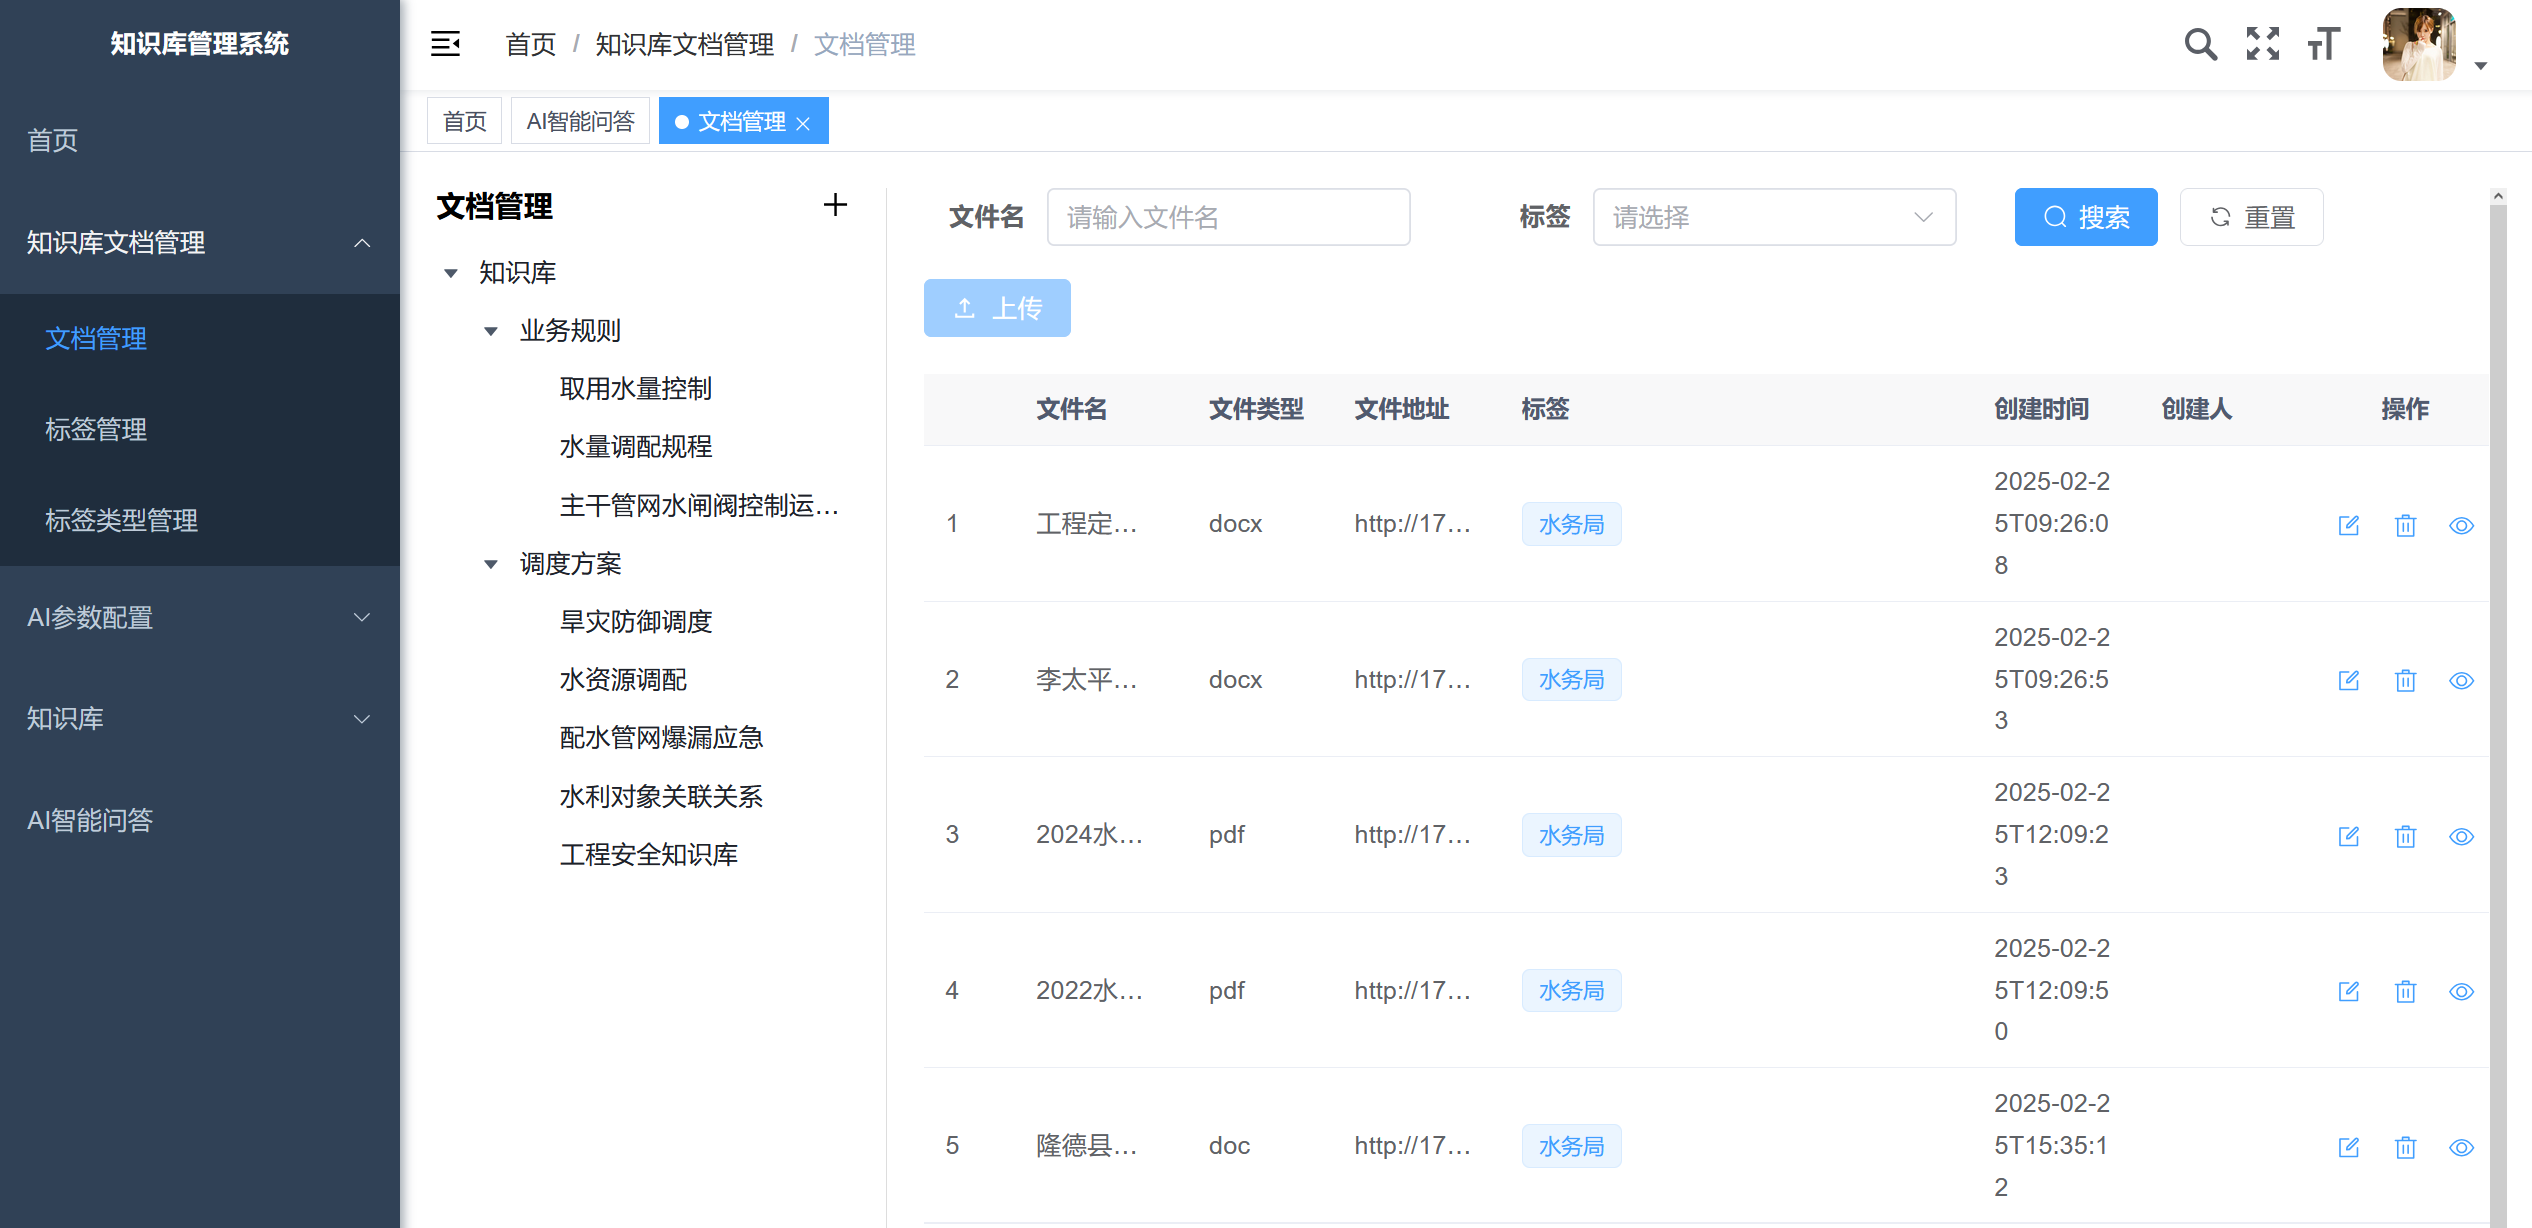
\includegraphics[width=0.91\textwidth]{知识库管理界面.png}
    \bicaption[知识库管理界面]{知识库管理界面}[Knowledge base management interface]{Knowledge Base Management Interface}
    \label{fig:知识库管理}
\end{figure}
\begin{figure}[!htbp]
    \centering
    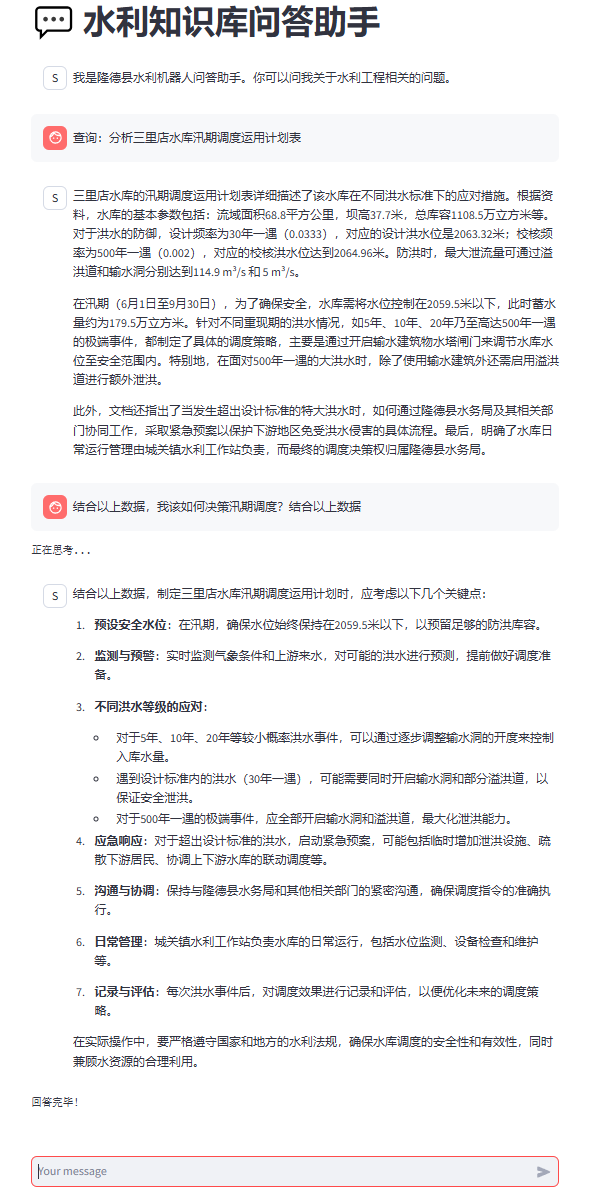
\includegraphics[width=0.75\textwidth]{多轮回答.png}
    \bicaption[多轮问答功能]{多轮问答功能}[ Multi round Q\&A function]{ Multi Round Q\&A Function}
    \label{fig:多轮对话展示}
\end{figure}

下面通过图\ref{fig:单轮问答}、图\ref{fig:结构化数据}和图\ref{fig:多轮对话展示}展示了表格数据推理框架在实际应用中的对话效果以及针对知识库的智能问答反馈系统的界面展示。其中,图\ref{fig:单轮问答}呈现了表格的单轮问答效果,当系统识别到表格信息时,会将Agent输出的database表格展示在界面中,并支持对展示表格的保存功能。图\ref{fig:多轮对话展示}则展示了在多轮对话场景下系统的推理结果,这些结果由通用大模型根据上下文中的本地知识进行分析后生成。图\ref{fig:结构化数据}展示了当检索返回的表格为结构化数据表格时的推理结果,从回答中可以看出,大模型对JSON形式的结构化数据具备良好的推理能力。

\begin{figure}[htb]
    \centering
    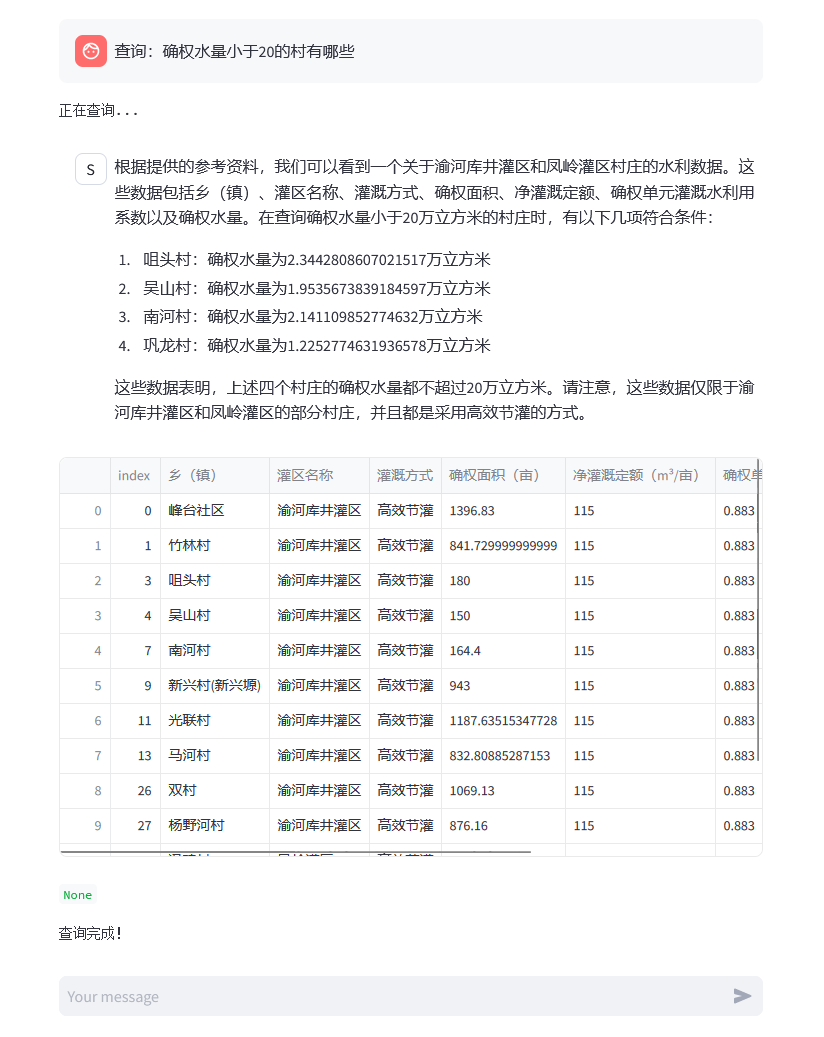
\includegraphics[width=0.82\textwidth]{单轮问答表格推理.png}
    \bicaption[单轮问答表格推理]{单轮问答表格推理}[Offline Database File Upload Function]{Offline Database File Upload Function}
    \label{fig:单轮问答}
\end{figure}
% 在单轮的查询过程中,反馈系统会将全部符合条件的表格数据返回给用户,并通过表格展示的方式,将表格数据以可视化的形式展示给用户。用户可以通过点击表格中的链接,查看表格的详细内容。同时对表格内容含义等相关信息进行解释说明。
% 在多轮对话的过程中,反馈系统会根据用户的提问,从上下文和知识库中检索需要信息进行进一步推理,提出更准确的专家意见与决策,生成更高质量的回答。
在智能反馈交互系统中,单轮查询与多轮对话是两种主要的交互模式。在单轮查询过程中,反馈系统将符合查询条件的所有表格数据完整地返回给用户。为了增强数据的可读性与用户体验,系统采用表格展示的方式,将数据以结构化的形式呈现,使用户能够清晰地浏览各项信息。此外,为了满足用户深入了解数据的需求,表格中的特定元素被设计为可点击的链接。用户通过点击这些链接,可以将召回的表格以excel格式下载保存,从而获取表格中各项数据的详细内容。系统还配备了相应的解释说明功能,对表格中数据的含义、背景以及相关关联信息进行解读,帮助用户全面理解数据所传达的信息。
而在多轮对话场景下,反馈系统则需要具备更强的逻辑推理与信息整合能力。随着对话的深入,用户的问题往往更加复杂且具有上下文依赖性。此时,反馈系统不仅要关注当前提问,还需将之前的对话内容作为重要的参考依据,同时深度挖掘知识库中的相关知识,通过复杂的语义分析与逻辑推理,将新获取的信息与已有信息进行融合,从而提出更加精准、更具专业性的专家意见与决策建议。
\begin{figure}[ht]
    \centering
    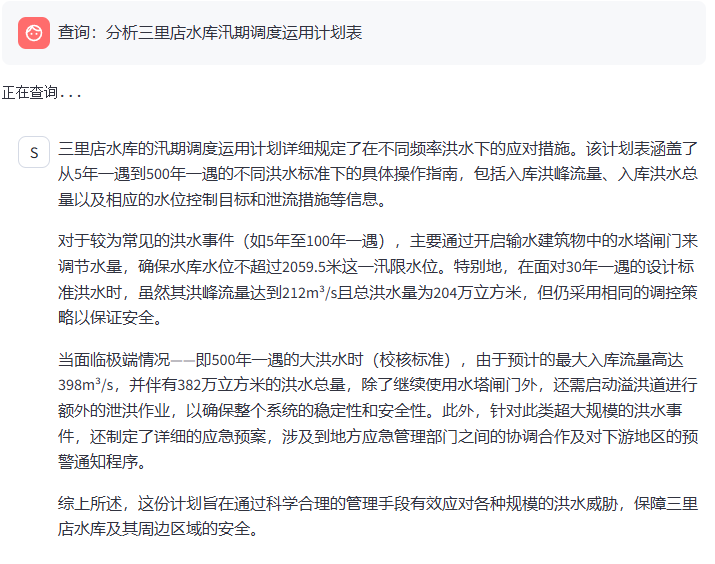
\includegraphics[width=0.74\textwidth]{结构化数据处理功能.png}
    \bicaption[结构化数据处理功能]{结构化数据处理功能}[Structured data processing function]{Structured Data Processing Function}
    \label{fig:结构化数据}
\end{figure}


\section{本章小结}
本章聚焦于第\ref{cha:第四章}章提出的技术框架在水利领域智能反馈交互系统中的设计,系统关键技术框架构建方面,基于LangChain框架与FAISS向量数据库,设计并实现了高效的检索增强生成(RAG)问答系统。通过整合多级表格数据检索、大模型推理优化及用户交互界面,构建了完整的端到端技术链路,显著提升了系统对结构化数据的处理能力与响应效率。RAG问答反馈功能优化方面,针对水利领域专业知识的封闭性与复杂性,提出多级表格数据检索方法,通过表头与表名的向量化存储策略,解决了传统文本切块导致的表格信息失真问题。结合循环推理框架与Agent代理思想,将复杂表格任务分解为SQL生成与执行的多步流程,有效弥补了大模型在数值推理与长上下文处理中的局限性,提升了回答的准确性与可解释性。

知识库管理功能实现方面,设计并开发了知识库的动态管理功能,支持用户对本地文件的查询和浏览。通过JSON与SQLite的三级存储结构,实现了结构化表格数据的高效存储与快速检索,确保系统在水利调度场景下的灵活性与可扩展性。实际应用与效果验证方面,通过实际案例展示了系统在单轮问答、多轮对话及结构化数据处理中的表现。实验结果表明,反馈系统能够准确召回本地知识、生成专业建议,并通过流式输出与交互式界面优化用户体验,为水利从业人员提供了高效、可靠的技术支持。本章内容不仅验证了检索增强生成技术与Agent框架在垂直领域中的实用价值,也为后续智能化问答系统的设计与行业落地提供了重要参考。

本章主要内容以作者在合作企业进行实习期间所撰写的实习报告形式提交,该知识库的智能反馈交互系统已在隆德县水利局正式上线并投入使用。

% !Mode:: "TeX:UTF-8"
\chapter{总结与展望}
\label{cha:第六章}
\section{全文总结}
本文围绕基于大模型的智能反馈交互系统的核心技术与应用展开系统性研究,重点突破模型轻量化压缩、表格数据推理优化及垂直领域系统集成等关键问题,主要取得以下成果:    1、针对一种文本编码网络——循环神经网络,提出一种基于本征正交分解(Proper Orthogonal Decomposition, POD)的动力学系统模型压缩方法,通过循环神经网络隐藏状态的低维投影,将模型参数量与计算量分别压缩至原始模型的34.4\%与25.6\%,精度损失控制在5\%以内,并将传统动力学方法引入神经网络中,提高了其可解释性。
2、针对大模型对结构化表格数据推理的局限性,设计多级表格检索和推理框架,结合Agent代理思想及SQL代码生成技术,将复杂数值计算转化为可执行程序,并构建检索-优化-生成的循环自纠错机制,优化生成质量。
3、针对数字孪生灌区目前存在的智能反馈交互系统缺失。无法适应调度系统升级需求等问题,设计并实现了数字孪生灌区多功能知识库,结合RAG技术为智能反馈交互系统提供本地知识支撑。通过建立业务规则库来支撑业务场景的规则适配,规范和约束水利业务管理行为。
4、为验证基于本征正交分解的动力学系统模型压缩方法、多级表格检索和推理框架等方法在实际场景中的优化效果,设计并实现了基于知识库的智能反馈交互系统。提高了知识库的利用效率和水利水库调度领域的智能化水平。将检索增强生成技术与本地知识库技术结合并成功应用于水库调度、灌溉管理等场景。系统支持流式输出与多轮交互,形成可复用的行业解决方案。研究通过理论创新与工程实践的结合,验证了大模型在知识密集型任务中的潜力,为智能系统的开发与垂直领域应用提供了方法论支撑与实践范例。
\section{未来研究展望}
本文及相关研究在该领域中仍然存在许多不足,作者认为还存在以下几个方面后续需要进一步扩充和深入研究:

1.	在动力学系统下的模型压缩方法方面,本文提出的基于POD的压缩方法在模型适用性上存在一定的局限性,目前仅在RNN类网络中得到了成功应用。未来研究应进一步探索POD方法在应用更为广泛的Transformer模型中的适用性,通过相关研究验证其在Transformer模型下的合理性和有效性。同时,应积极推动更多动力学系统解决方案向神经网络领域的迁移,以拓展神经网络在动力学系统中的应用范围和效果。

2.	针对表格数据的大模型推理问题,目前主流方法在SQL生成的成功率上仍有待提高。未来可以通过指令微调等多种方式,优化大模型对SQL指令的生成过程,提高其生成准确率。具体而言,可以通过对模型进行针对性的训练和优化,使其更好地理解和生成SQL指令,从而提升表格数据推理的准确性和效率。

3.	在实际的反馈系统开发中,时效性是一个关键因素。目前对于系统的并行功能开发及计算资源的合理分配,以及多模态输入的扩展等方面,还存在一定的研究空间。未来应进一步研究如何优化系统的并行功能,合理分配计算资源,以提高系统的响应速度和处理能力。同时,应拓展多模态输入的支持能力,使系统能够更好地处理多种类型的数据输入,提升用户体验和系统性能。

\listoffigures                        % 插图索引
\listoftables                         % 表格索引

% 参考文献. 
\bibliographystyle{gbt7714-numerical}
\bibliography{reference/refs}

\begin{publications}


{\heiti 一、论文}

[1] ***, ***, ***. A Sequence Model Compression Method Based on Proper Orthogonal Decomposition[C/OL]//2023 3rd International Conference on Computer Science and Blockchain (CCSB). 

{\heiti 二、专利}

[1] 基于本征正交分解的循环神经网络的压缩方法、装置、处理器及其计算机可读存储介质.****. ***,***,***,***. CN202310814136.5[P]. 2023-08-14.


{\heiti 三、项目}

[1] 科技创新2030-“新一代人工智能”重大项目“人工智能平台互联互通标准与评测技术研究” 2021ZD0110600,参与

[2] 基于大语言模型的数字孪生灌区知识库研究及开发,参与


\end{publications}
           % 发表论文清单
% 致谢
\begin{acknowledgement}
  衷心感谢导师 xxx 教授对本人的精心指导. 

  \vspace{50bp}

  \hfill ***

  \hfill 上海大学

  \hfill 2025 年 3 月 14 日

\end{acknowledgement}
        % 致谢

\backmatter
\begin{appendix}
\chapter{经典不等式}
论文中用到的经典不等式.\\

\noindent{\bfseries (H\"older Inequality)}
设~$a_i\geq0$, $b_i\geq0$, $i=1$, $2$, $\cdots$, $n$, 且~$p>1$, $q>1$ 
满足~$1/p+1/q=1$. 则有
\[
\sum_{i=1}^{n}a_ib_i\leq\left(\sum_{i=1}^{n}a_i^p\right)^{\frac1p}
\cdot\left(\sum_{i=1}^{n}b_i^q\right)^{\frac1q},
\]
等号成立当且仅当存在一个常数~$c$ 满足~$a_i^p=cb_i^q$.\\

\noindent{\bfseries (PM Inequality)}
设~$x_1$, $x_2$, $\ldots$, $x_n$ 是~$n$ 个非负实数. 如果~$0<p<q$, 那么
\[
\left(\frac{x_1^p+x_2^p+\cdots+x_n^p}{n}\right)^{\frac{1}{p}}\leq
\left(\frac{x_1^q+x_2^q+\cdots+x_n^q}{n}\right)^{\frac{1}{q}},
\]
等号成立当且仅当~$x_1=x_2=\cdots =x_n$.\\

\noindent{\bfseries (AM-GM Inequality)}
设~$x_1$, $x_2$, $\ldots$, $x_n$ 是~$n$ 个非负实数. 则有
\[
\frac{x_1+x_2+\cdots+x_n}{n}\geq\sqrt[n]{x_1x_2\cdots x_n},
\]
等号成立当且仅当~$x_1=x_2=\cdots =x_n$.
\end{appendix}

\end{document}
